% TO DO :
% Remove the graphs. Just keep this section theoritical with examples.
% This file contains description of the controller architecture.
\section{Memory Controller Design}
\label{sec:memcontrol}
The previous section describes various coding schemes to design the storage space of the proposed memory systems. In this section, we discuss the architecture of memory controller which constitutes the second main component of the memory system. Given that our memory system redundantly stores the data in memory banks, the design of the memory controller involves many novel ideas that enable it to exploit this redundancy in order to provide improved parallel access to the memory banks. This section presents these key architectural ideas behind the memory controller design along with various implementation related deails.
%The memory design involves two key components: 1) storage space comprising of memory banks and 2) memory controller 
%The coding schemes discussed in previous section is implemented using systemC. 
%This section describes the architectural detail of how the schemes are 
%implemented using optimized algorithms. \\
%In this section, we explore the technique of dynamic coding in order to reduce 
%the memory and access overhead
%associated with the parity banks. We first discuss the scheme of dynamic coding 
%and follow it by discussing the potential benefits of prefetching the codes.\\

\subsection{Main units at memory controller}
A general memory controller consists of three main levels of processing (cf.~Figure~\ref{fig:pseudo-code}). The first level deals with handling the access requests from cores which is performed by {\em core arbiter}. The second level of processing is conducted by {\em bank arbiter} which is responsible for tracking requests for different data banks. The third main unit {\em access scheduler} deals with the final level of processing by scheduling the most efficient access patters for each memory clock cycle from the set of accesses {\color{red} assigned by the bank aribiter}. Next, we discuss all of these three units and their functions in a greater detail.
%first level is {\em Core Arbiter }, the unit responsible for handling requests 
%from cores.  The second level is {\em Bank Arbiter} responsible for arbitrating 
%requests to banks.  The third level is {\em Access Scheduler} which schedules 
%most efficient access for each cycle.\\
%%-----------------------
\begin{figure}[htbp]
\centering
	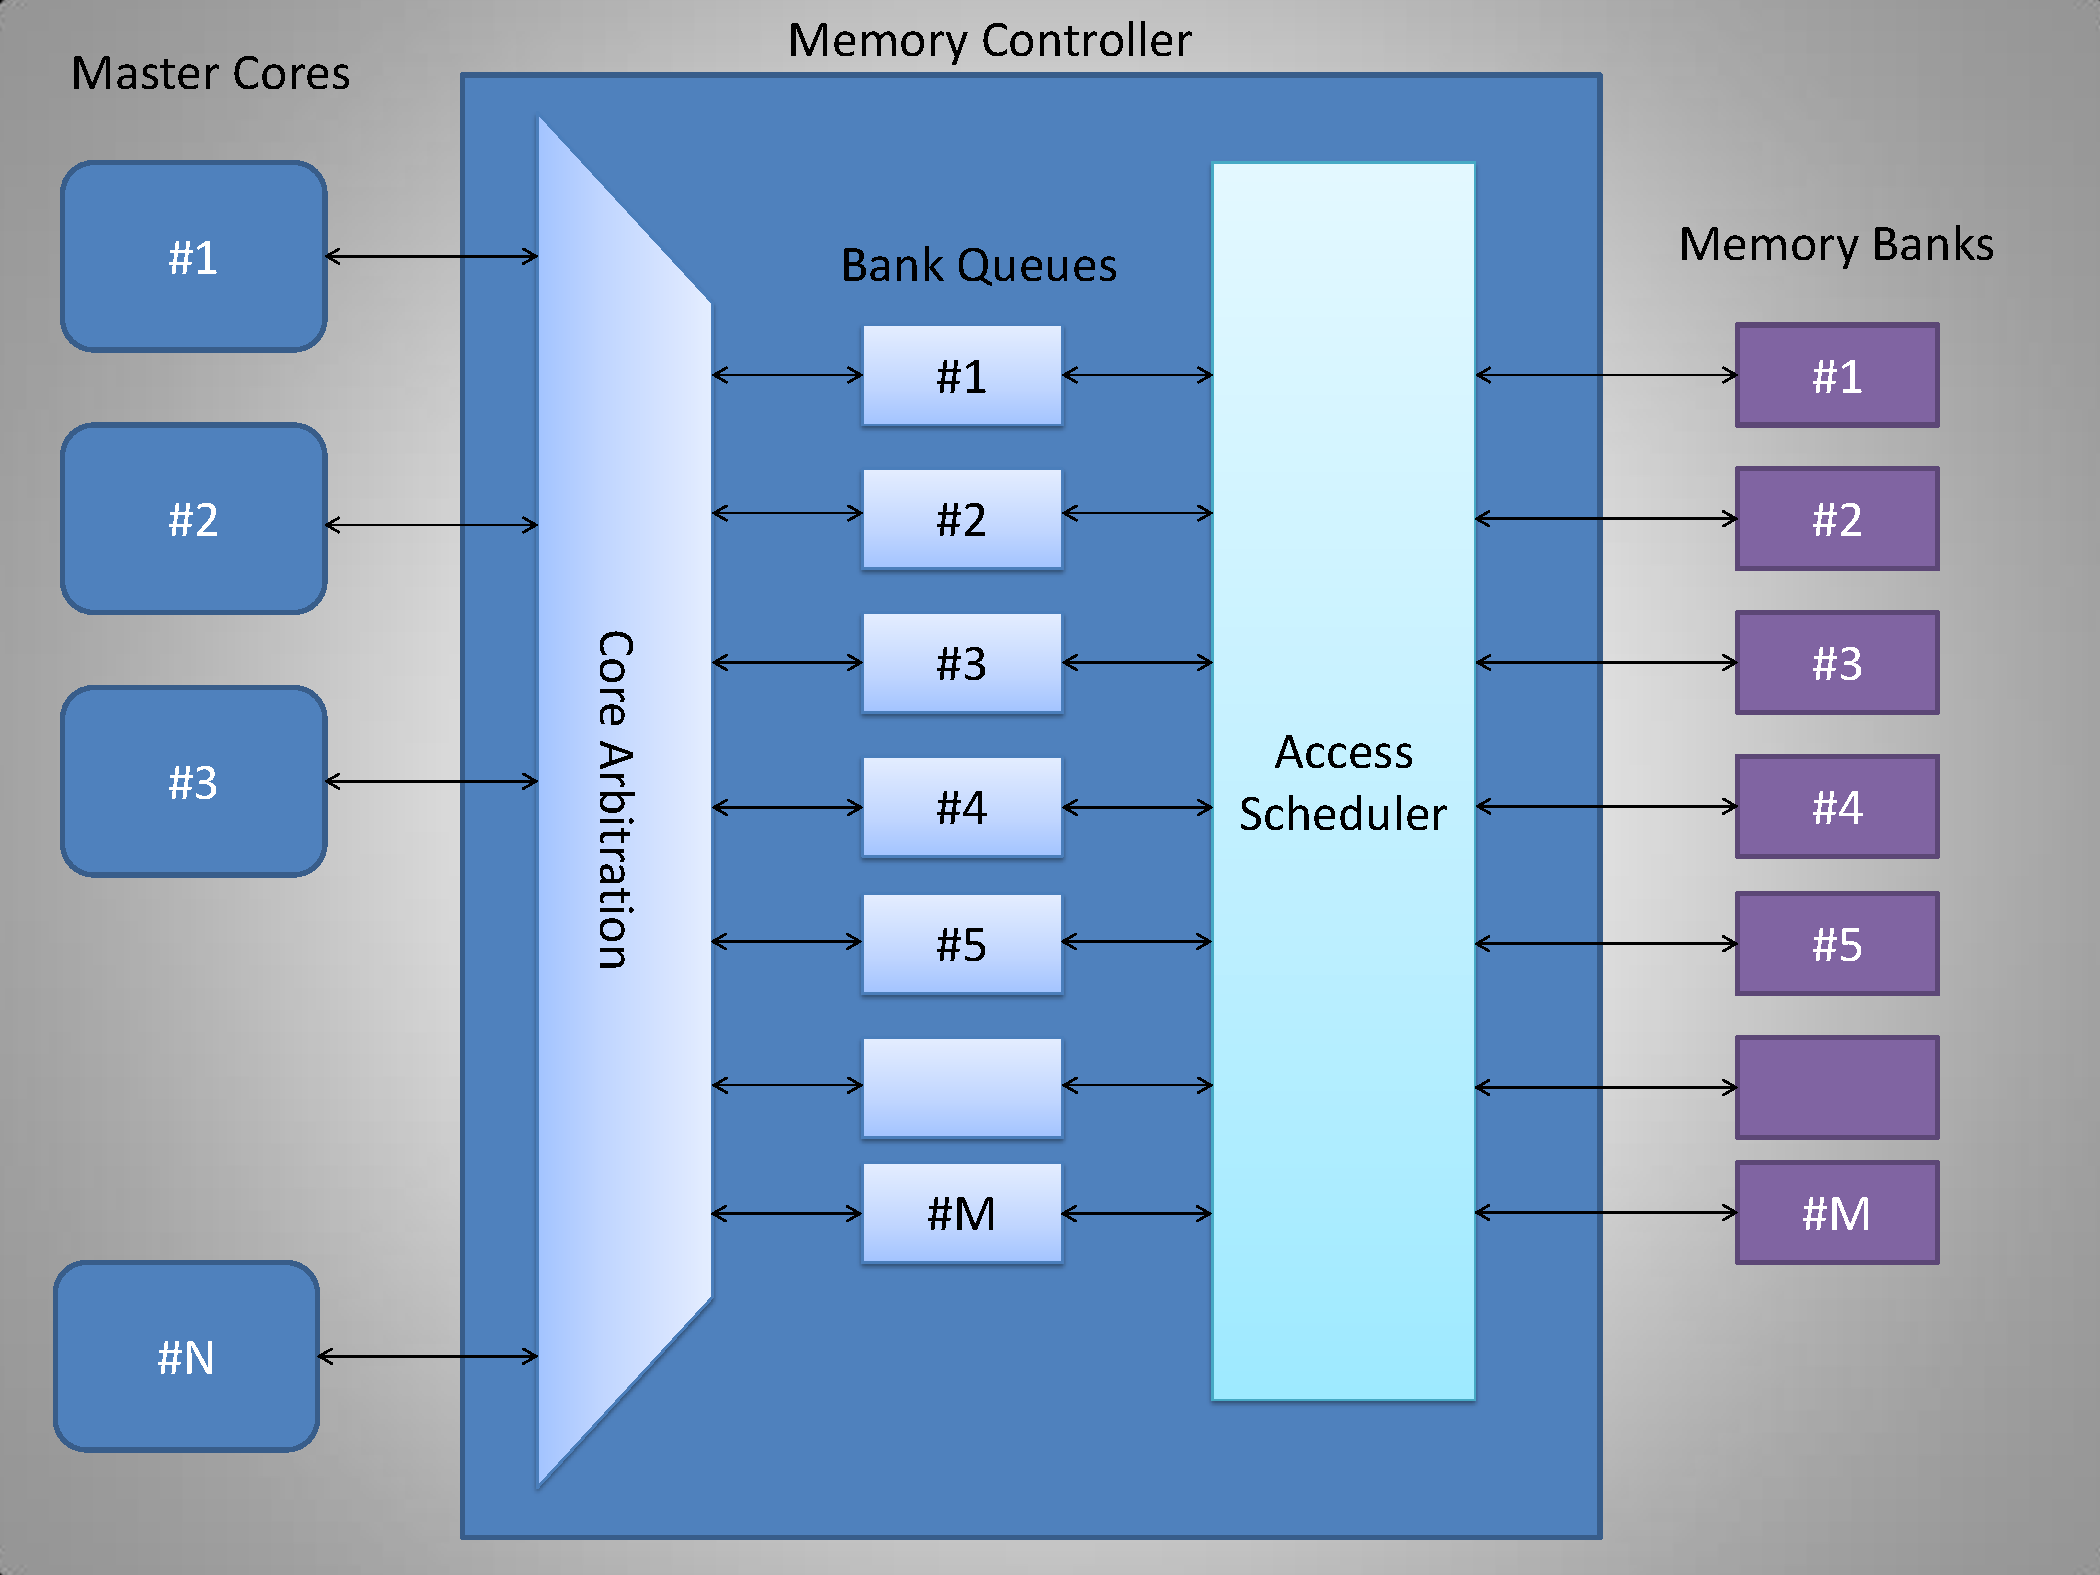
\includegraphics[width=0.7\linewidth]{fig/controllerArchitecture.pdf}
\caption{
{Architecture of Memory Controller} }
\label{fig:pseudo-code}
\end{figure}
%-------------------------
\begin{itemize}
\item \textbf{Core arbiter:~}The {\em core arbiter} receives request from all the cores at every clock cycle.  
It maintains a queue for each core. The depth of each queue is {\em 8 requests}.  
That is, it can hold 8 requests from each core for service. When a queue is 
filled up, the controller signals the respective core as busy. So, the core 
cannot issue a memory request and hence stalls until the controller's status 
gets back to normal. This unit is also responsible for arbitration among the 
request for cores. The arbitrator goes through the last element of each queue 
and determines the priority order. It uses a two-step priority order mechanism:
1) First, it arranges the request in order of QoS with high QoS at high 
priority; and  2) {Second}, for request having same priority, it arranges them using 
round robin.
\item \textbf{Bank arbiter:~}This unit contains read  and write queues for each data bank. The core arbitrator arbitrates requests from 
cores, expands them and fills them in the bank queues. The depth of bank queues 
in current implementation is $10$. This means that the depth of each read 
and write queue is $10$. These queues are for each bank. In an eight bank system, 
there are total of eight read queues and eight write queues. This requires a 
total of $160$ requests to be stored in these queues.
\item \textbf{Access scheduler:~}The access scheduler is responsible for scheduling access to
various memory banks in the storage space at every clock cycle.  This logic looks at the read and write queues for 
each data bank and forms an access pattern which is most efficient. In doing so, it 
goes through the requests in the bank and makes the pattern. It prioritizes the
requests at the bottom of the queue however, in case of coding memory systems 
(discussed in \ref{sec:readCodingAlgo}) it looks ahead in the queue to maximize 
the accesses per cycle. The write queues hold the writes until the writes are 
full. The reads are given priority over writes until the write queue gets 
filled.
\end{itemize}

{\color{red} We note that the first two components of the memory controller, i.e., core arbiter and bank arbiter, in the setting with coded memory banks should not differ much from those in the traditional setup with uncoded storage space. It's the third component, access scheduler, that directly interacts with the array of memory banks and it should take the underlying coding scheme into account while scheduling both read and write requests.} In the rest of this section, we discuss various parts of the access scheduler in detail.

%-----------------------
\begin{figure}[tbp]
\centering
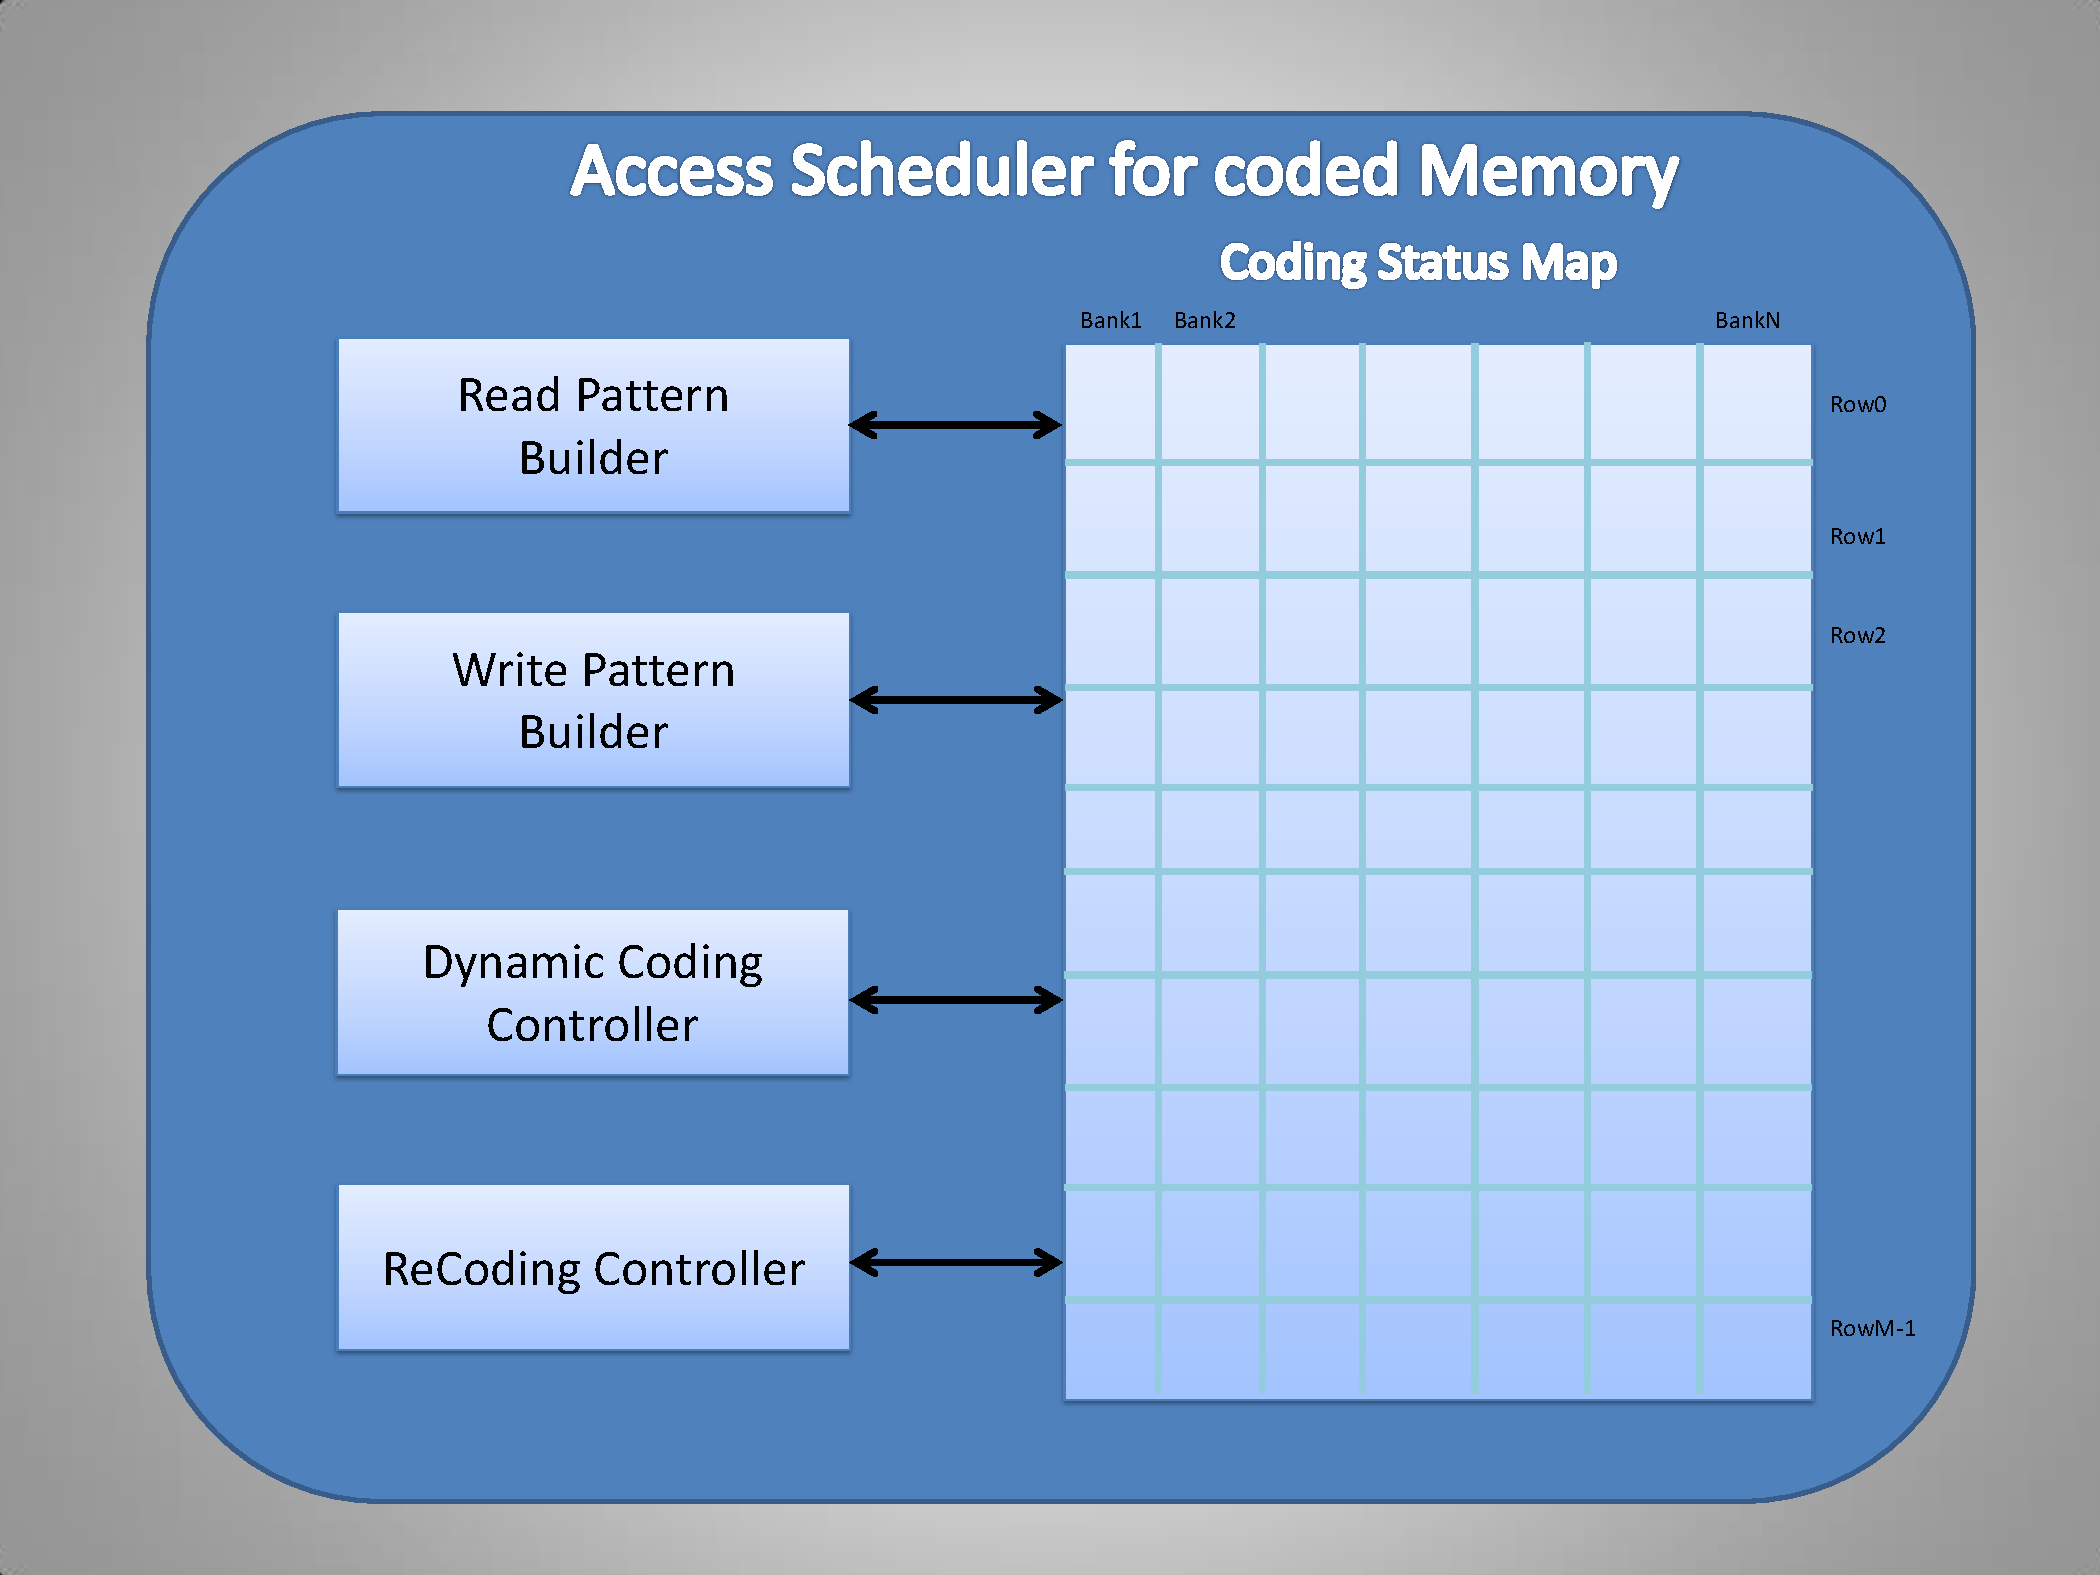
\includegraphics[width=0.7\linewidth]{fig/coded_access_scheduler.pdf}
\caption{
{Access scheduler for coded memory} }
\label{fig:coded_access_scheduler}
\end{figure}
%-------------------------
\subsection{Code Status Table}
\label{sec:codeStatusTable}
Due to write requests, the information stored in the memory banks need to be constantly updated. However, the updating an information element requires more work in the setup with coded memory banks as all the parity elements that depend on the information element also need be updated. In order to keep track of the freshness of the data stored in the various memory banks, we assign a storage space, namely {\em code status table}, in the access scheduler. As depicted in Figure~\ref{fig:coded_access_scheduler}, this block's rows correspond to rows of the memory banks. The different columns of the status table are associated to different memory banks in our memory design.  Each cell in the status table stores $2$ bits, which are mapped to the status of the code for the corresponding row of the memory banks as per Table ~\ref{table:codestatusmap}. We assume that the elements of the code status table are accessible at a very fast rate. %This memory is present in the memory controller and is assumed to be accessible at a very fast rate.


\begin{table}[h!]
	\centering
	\begin{tabular}{|c | c|}
\hline
00 &  {Codes are up-to-date}\\ \hline 
01 &  Codes are outdated. Fresh data in Data bank \\ \hline 
10 &  Codes are outdated. Fresh data in Parity bank \\ \hline 
11 &  Reserved \\
\hline
\end{tabular}
\caption{Code Status Map}
\label{table:codestatusmap}
\end{table}
%-----------------------
\begin{figure}[t!]
	%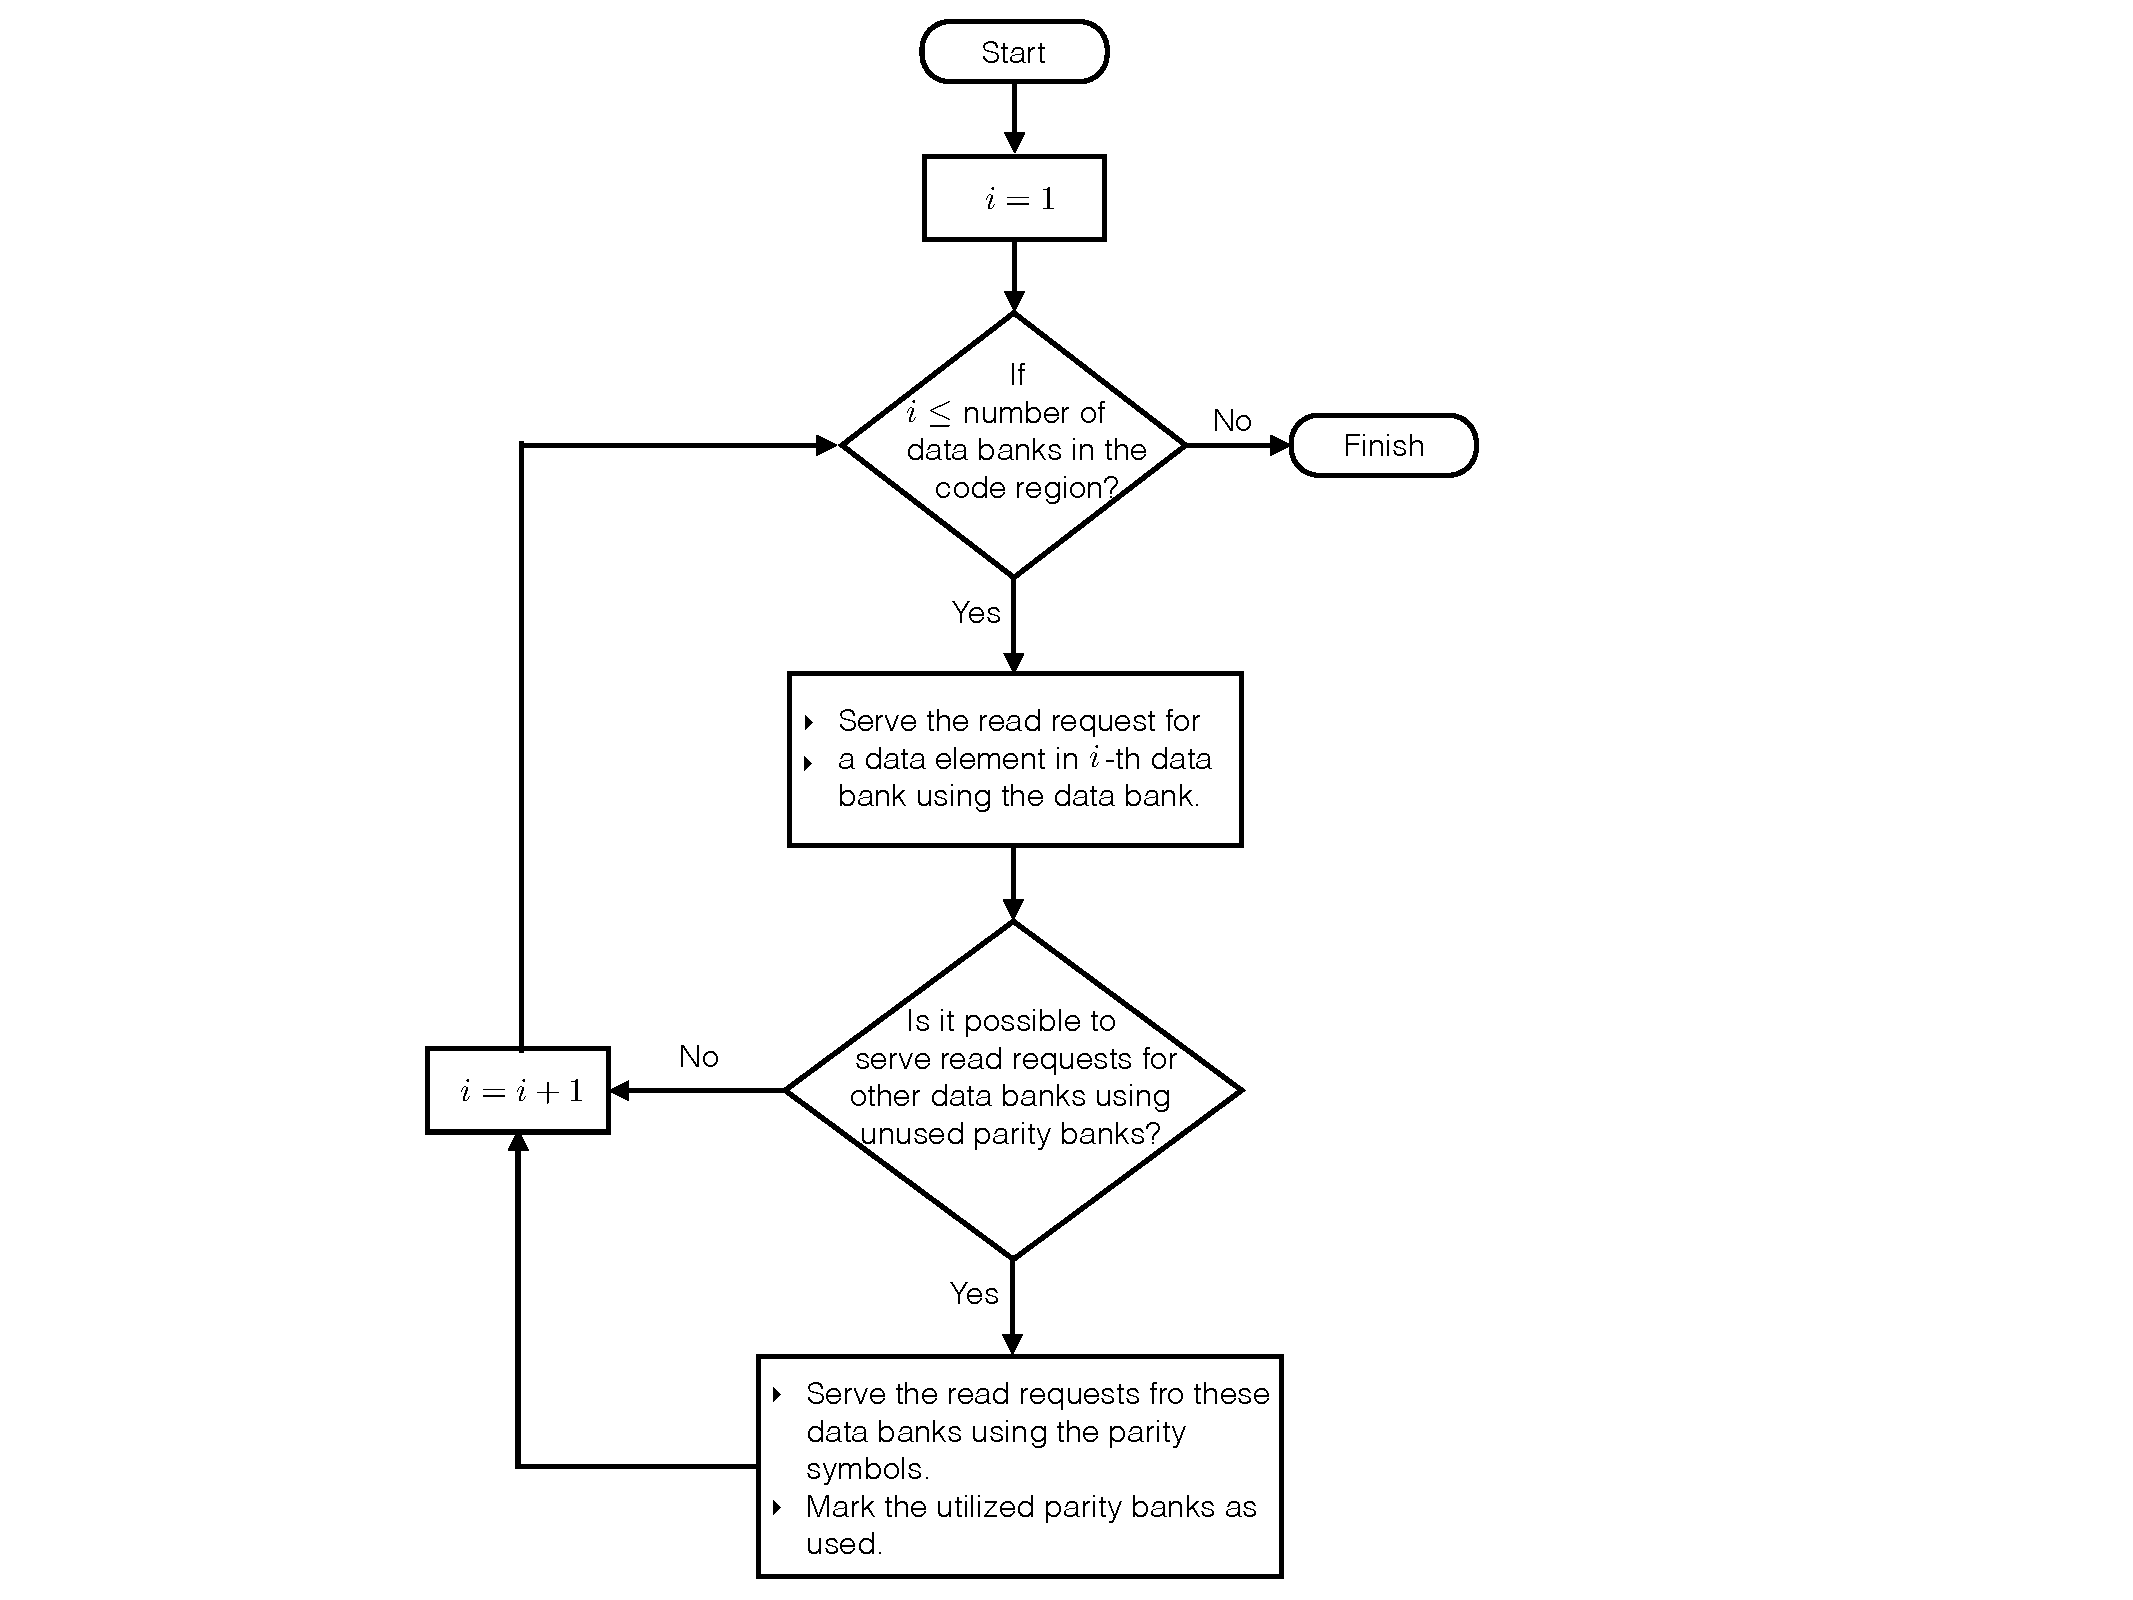
\includegraphics[width=0.9\linewidth]{fig/Read-algo.pdf}
	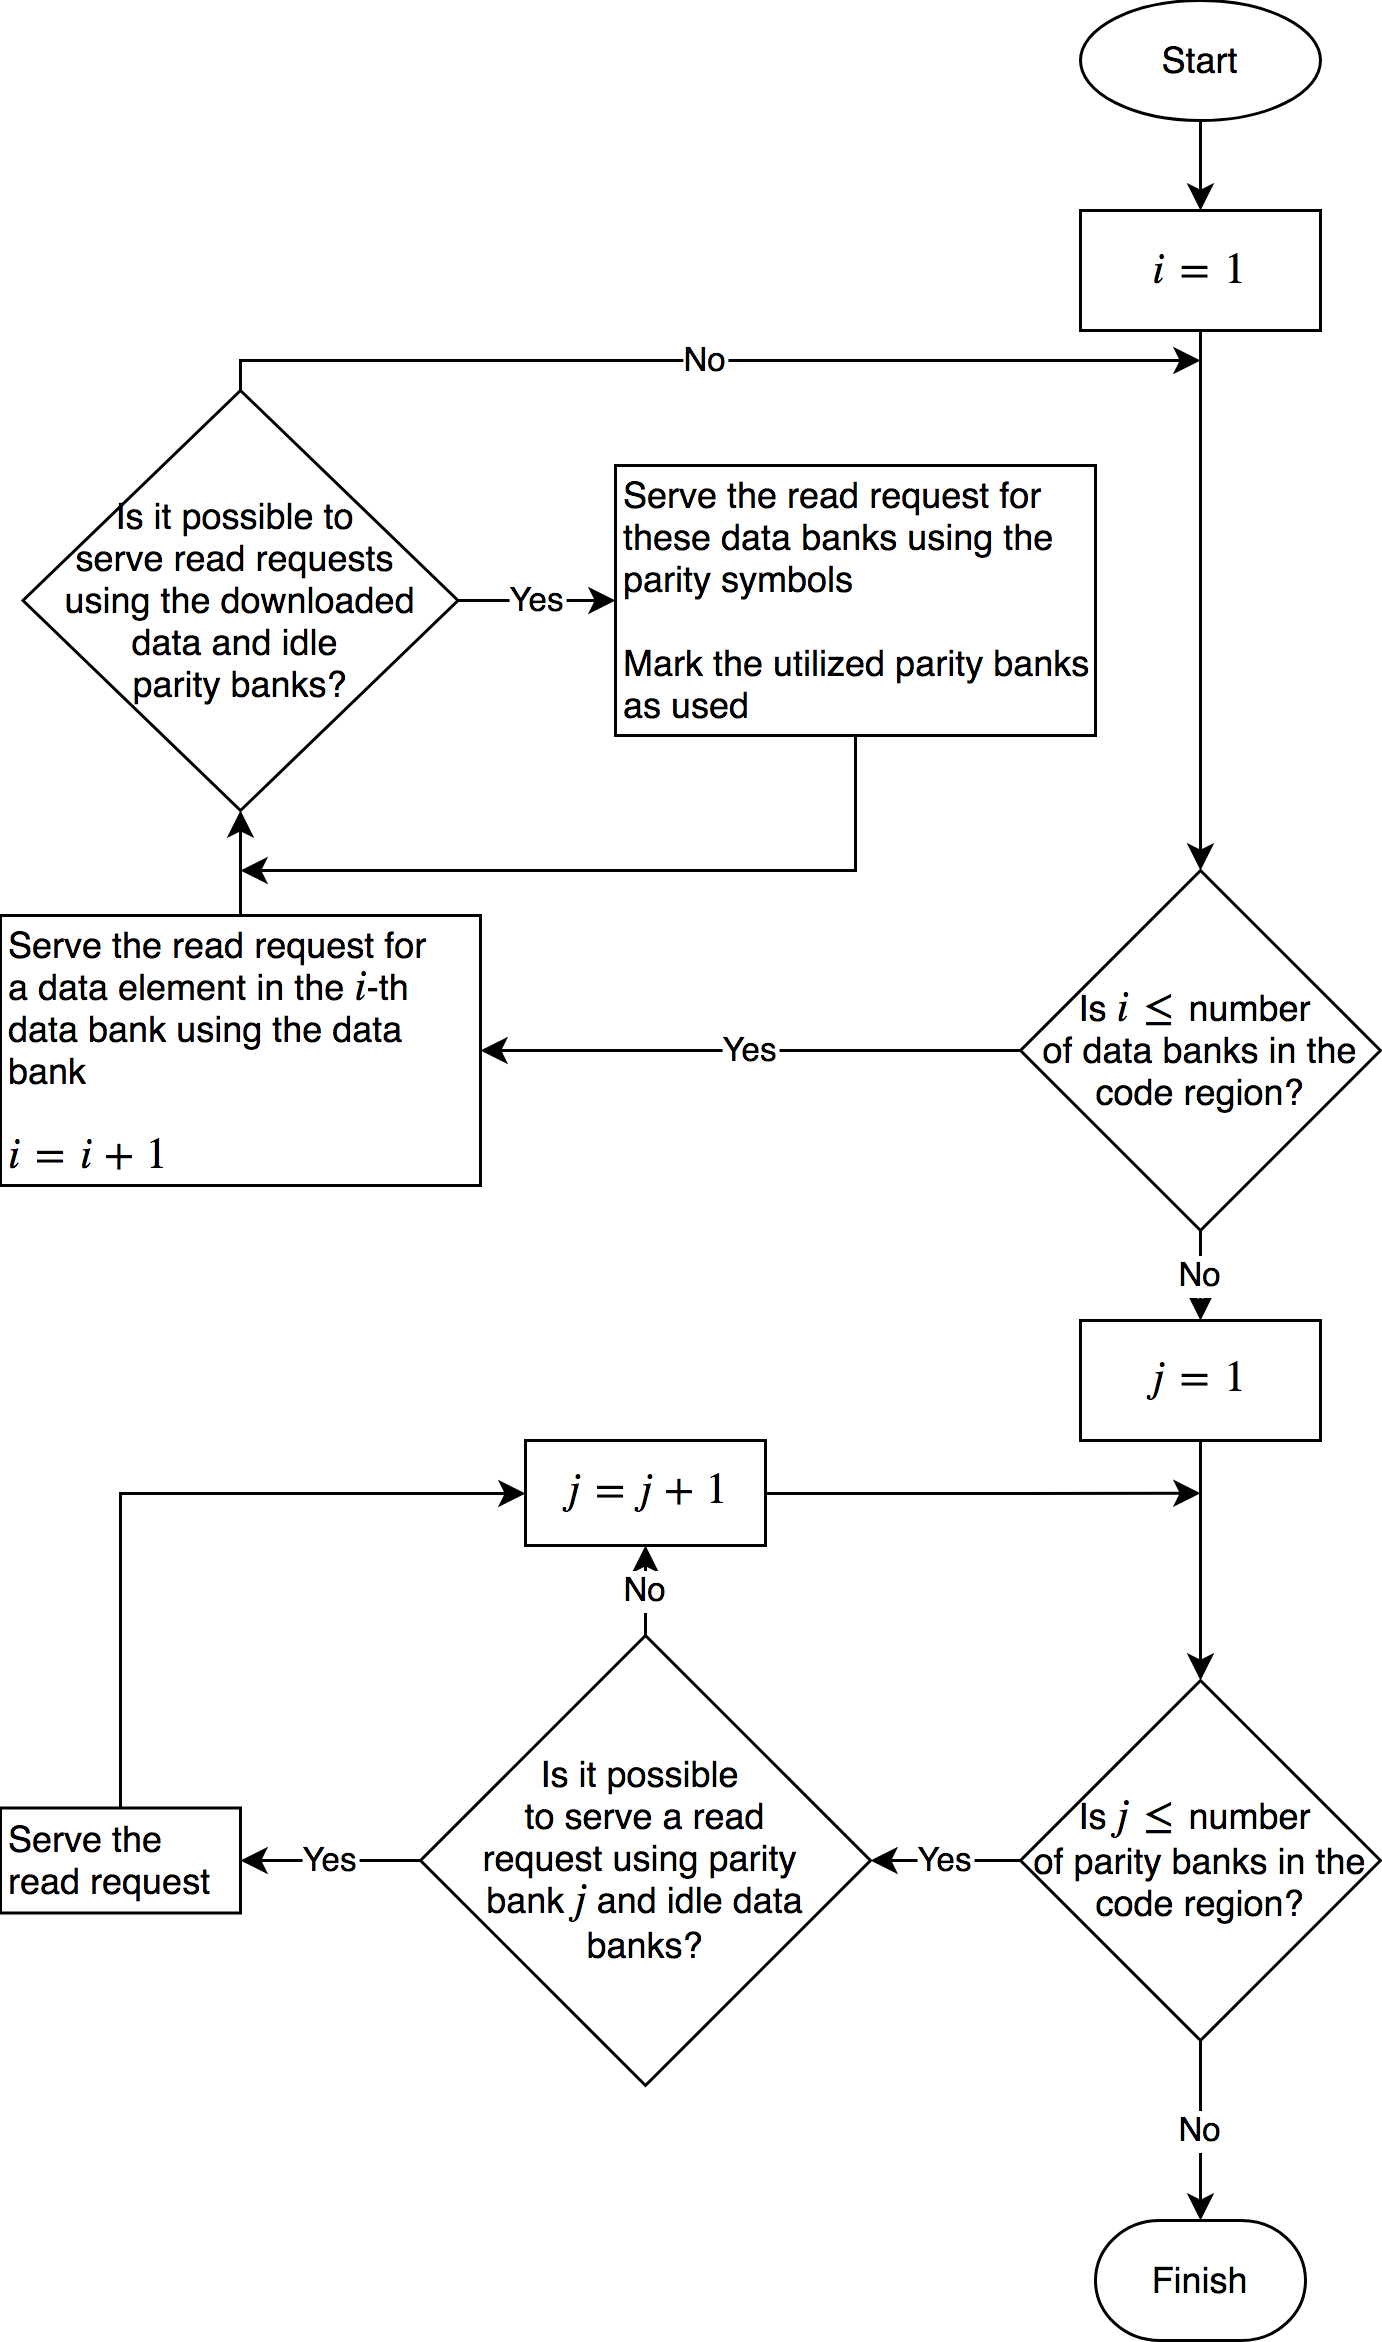
\includegraphics[width=0.96\linewidth]{fig/read_pattern_algo.png}
	\caption{{Description of the algorithm to build a read request pattern to be served in a given memory cycle.}}
	\label{fig:readAlgo}
\end{figure}
%-------------------------
%-----------------------
\begin{figure}[htbp]
	\centering
	%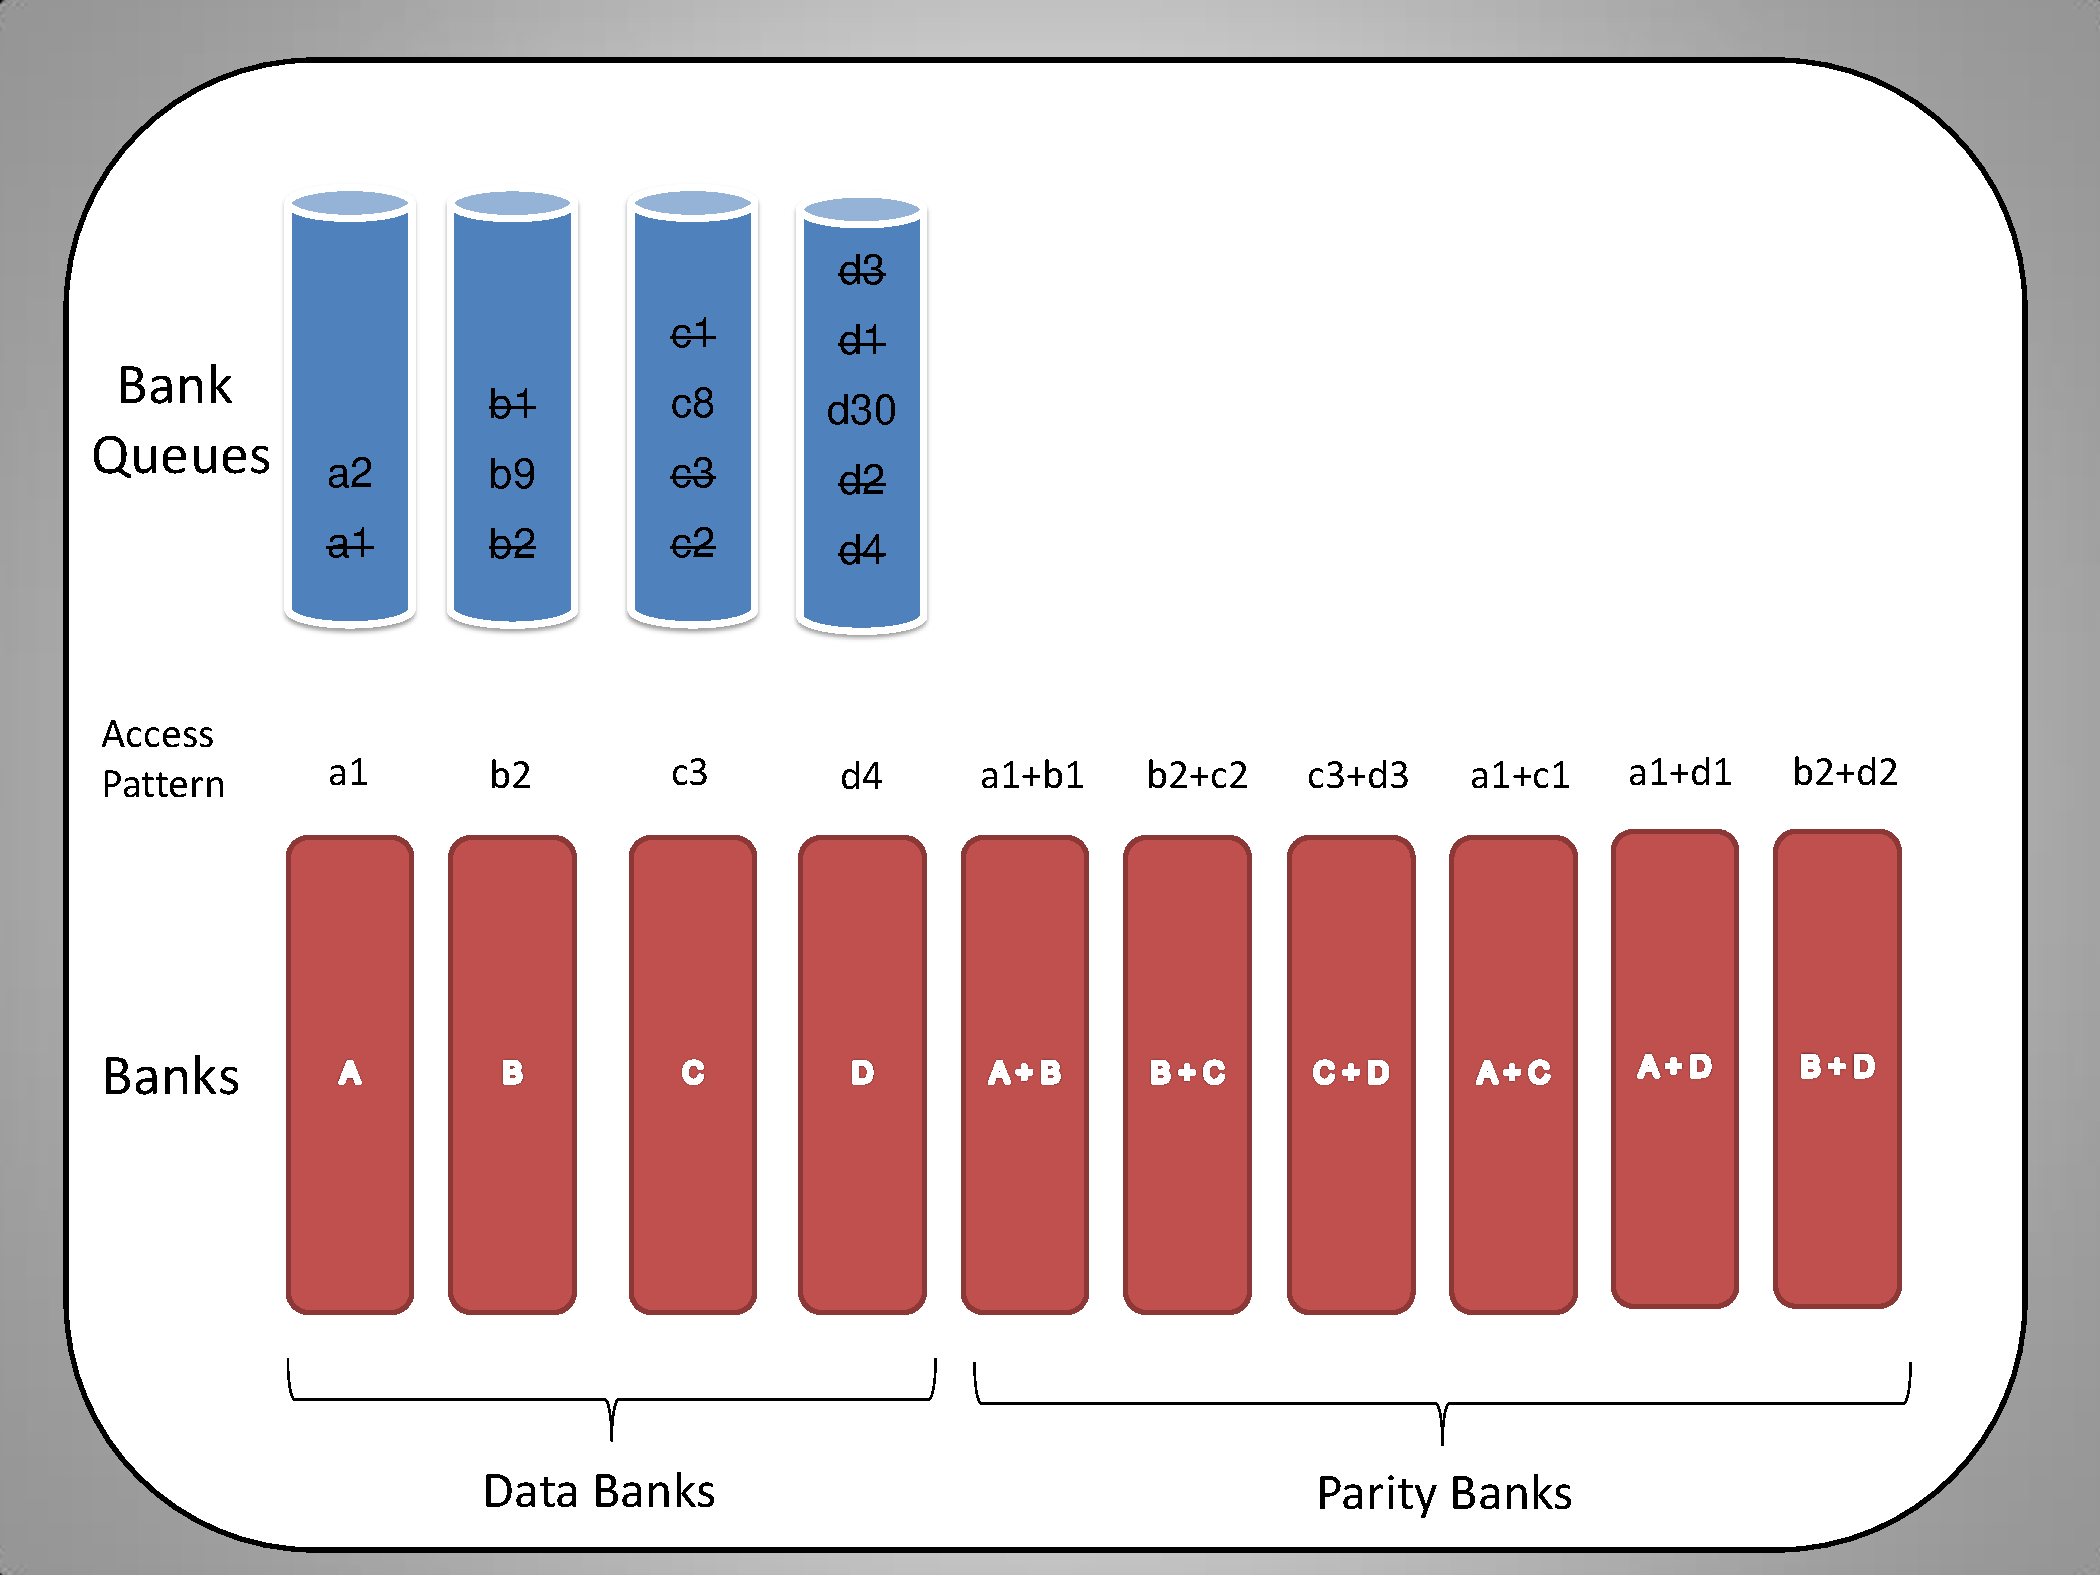
\includegraphics[width=0.7\linewidth]{fig/readAlgoAccessPattern.pdf}
	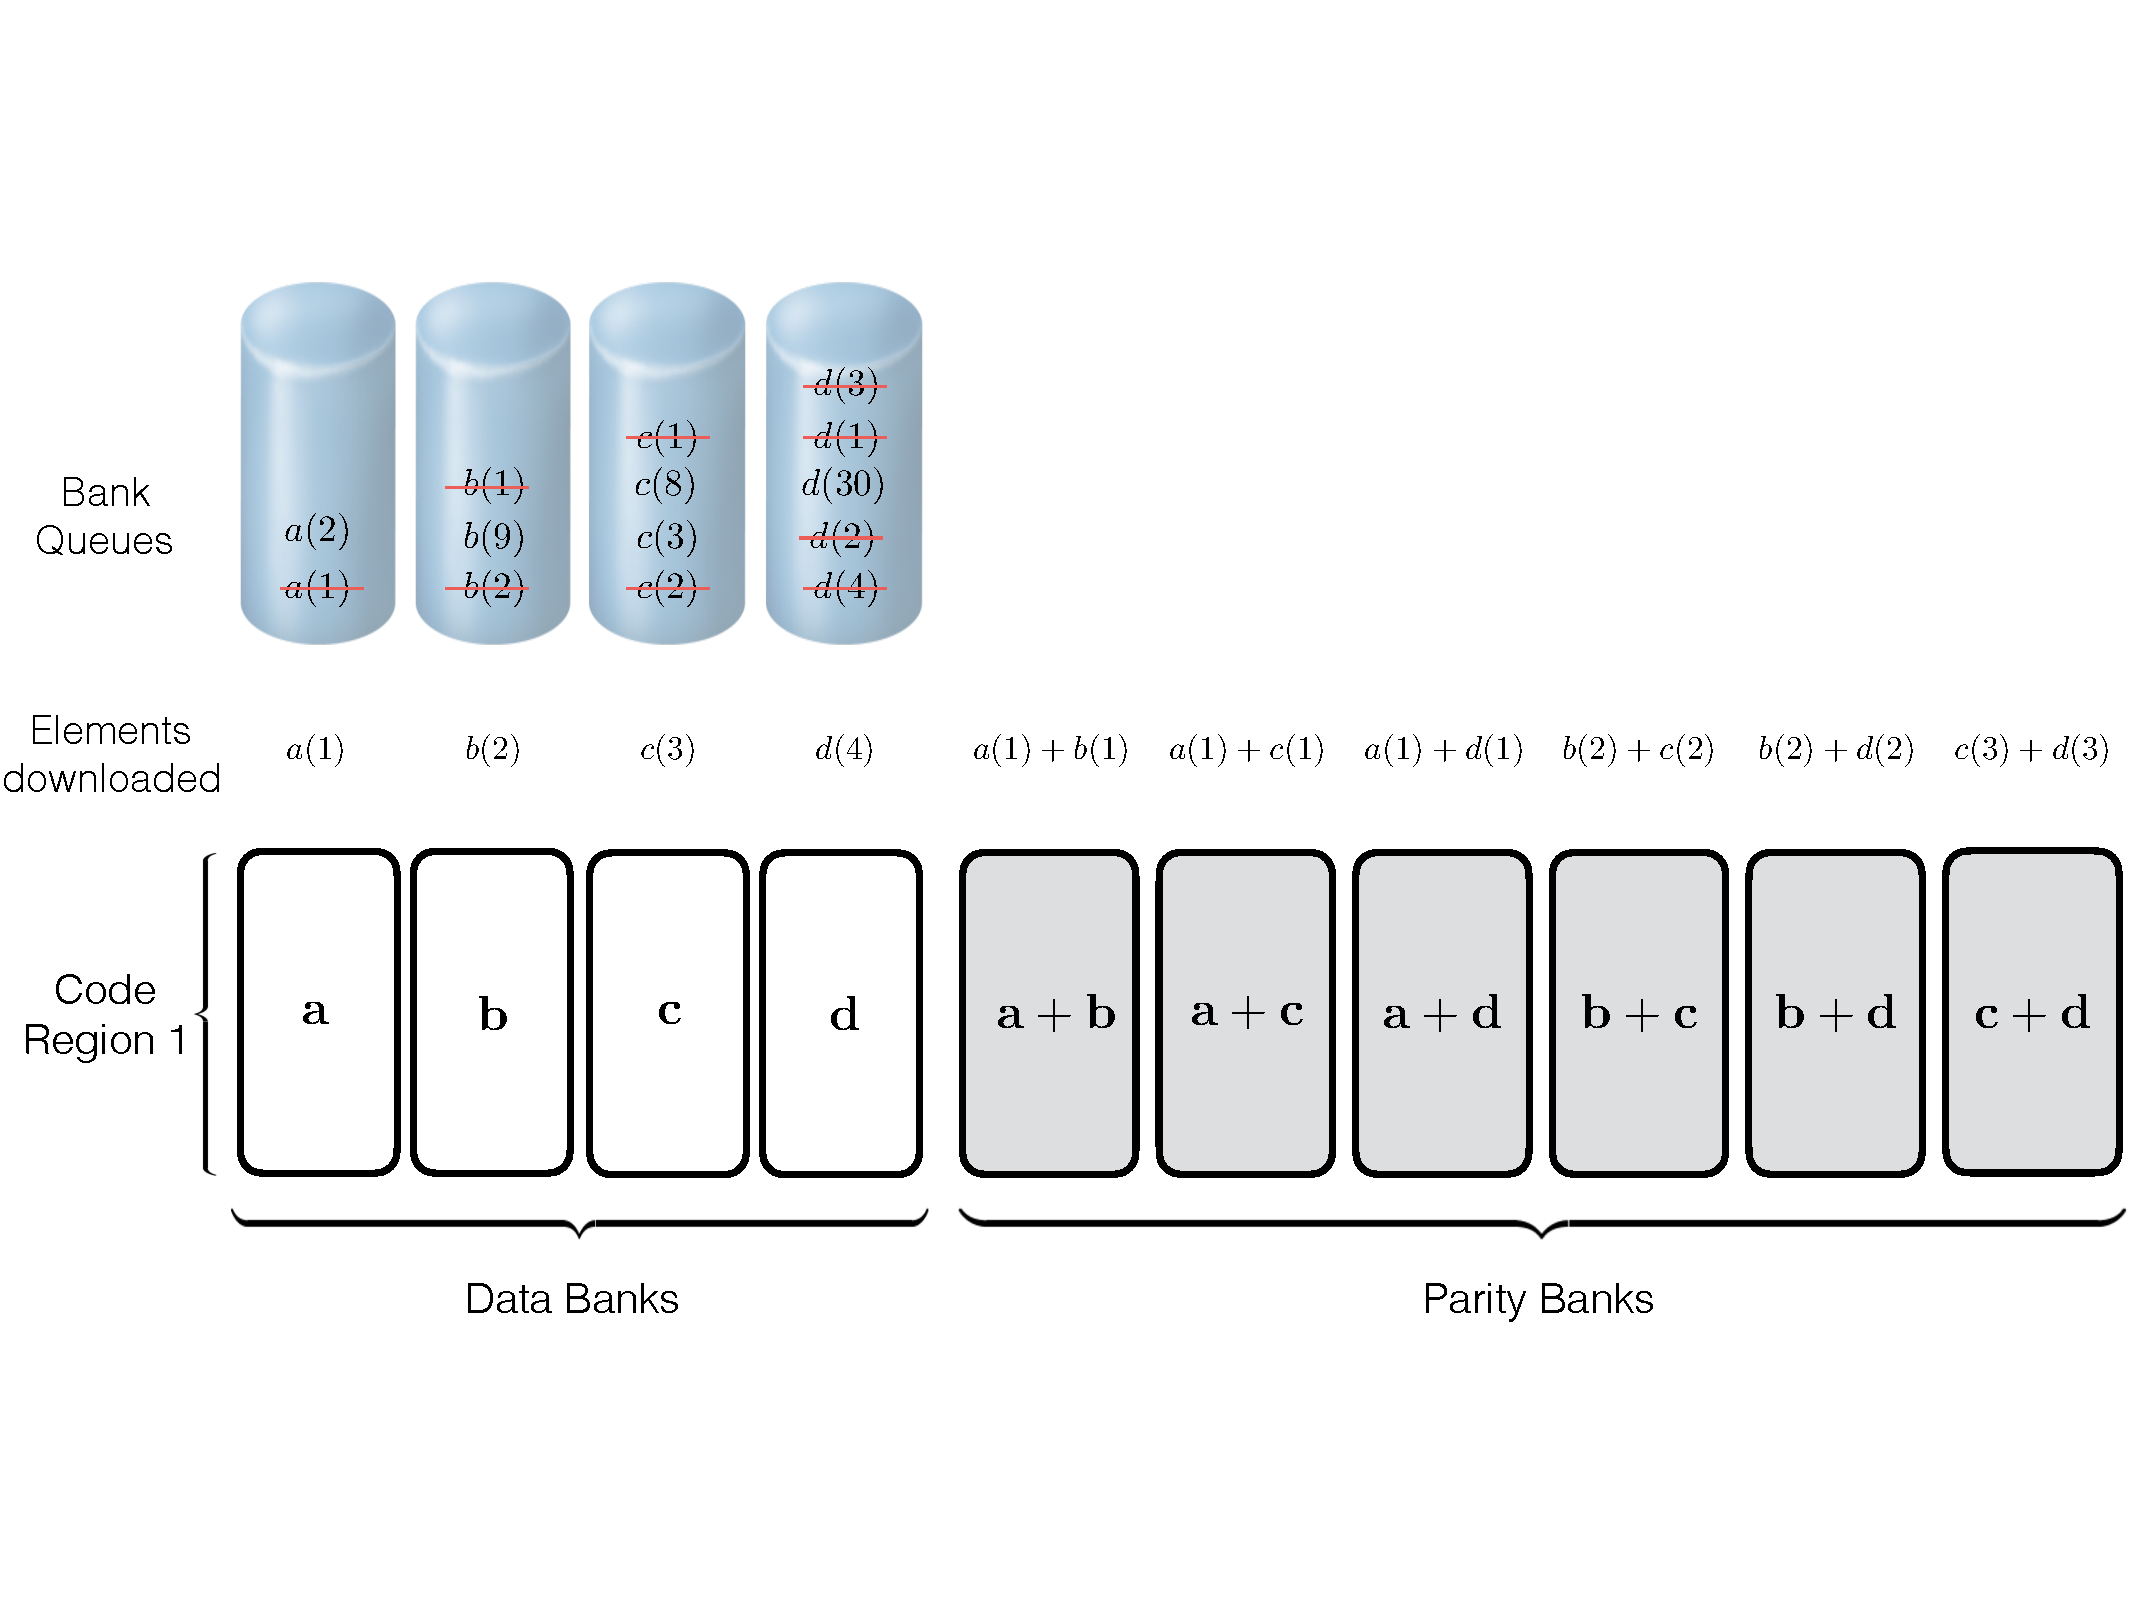
\includegraphics[width=0.96\linewidth]{fig/Read-Algo-Example.pdf}
	\caption{{Illustration of the algorithm to build a read request pattern to be served in a given memory cycle. All the read requests associated with the strikethrough elements are scheduled to be served in a given memory cycle. The figure also shows the elements downloaded from all the memory banks in order to serve these read requests.}}
	\label{fig:readAlgoAccessPattern}
\end{figure}
%------------------------
%\subsection{Read Algorithm for Coded Memory system}
\subsection{Read pattern builder}
\label{sec:readCodingAlgo}
The primary objective of the access scheduler it to maximize the number of read requests served in a given memory cycle. This is achieved by the block {\em read pattern builder}. The main idea here is to exploit the redundancy in the parity banks in order to serve as many simultaneous read requests as possible.

\Matt{We should include an example where using idle data banks is advantageous} We describe the algorithm employed by the read request pattern in Figure~\ref{fig:readAlgo}. We illustrate this algorithm with the help of an example, which is shown in Figure~\ref{fig:readAlgoAccessPattern}. %The accesses from parity banks is useful only if one of the corresponding access  is made to the data bank. Figure ~\ref{fig:readAlgo} describes the algorithm. Figure ~\ref{fig:readAlgoAccessPattern} describes an access pattern scenario. 
%The reads are maximized by using the parity banks. The key here is to be able to use the parity bank to serve the reads to other banks. 
The controller first marks {\em a(1)} to be read from the data bank $\mathbf{a}$. It then iterates through the read requests fro the data banks $\mathbf{b}, \mathbf{c},$ and $\mathbf{d}$ to find out if any of those requests can be served by combining $a(1)$ with parity elements from the unused parity banks. As it so happens, the read requests for $b(1), c(1)$ and $d(1)$ can be served using $a(1)$ and the parity banks. The controller marks the corresponding parity banks to be used (or busy). Then it moves to the data bank $\mathbf{b}$ to serves the read request for $b(2)$ using this bank. It then searches if it can serve any request for the elements in the data banks $\mathbf{a}, \mathbf{c},$ and  $\mathbf{d}$ by combining the downloaded data element $b(2)$ with the parity elements from the unused parity banks. As a result of this search, it decides to serve the read requests for $c(2)$ and $d(2)$ with the help of the (unused) parity banks storing the parity elements $b(2) + c(2)$ and $b(2) + d(2)$. Similarly, the read pattern builder goes through bank banks $\mathbf{c}$ and $\mathbf{d}$ to form the complete access pattern. As it can be observed from Figure ~\ref{fig:readAlgoAccessPattern}, the controller 
serves $4, 3, 2$, and  $1$ read requests for the data banks $\mathbf{d}, \mathbf{c}, \mathbf{b},$ and $\mathbf{a}$, respectively. The banks are thus 
accessed in order of their queue size with the least queue size accessed first 
for forming the access pattern. However, this rule does not always guarantee that 
there would be $1$ read requests for the first bank and $4$ access for the last bank. This 
is dependent on the actual read requests present in the queues. \Ankit{Also, we need to make sure that we are not jumping any write request while going through the queues to build a pattern, right? Or are we only doing FIFO processing of the read requests?}
\Matt{The Core arbiter should be designed such that jumping write requests is impossible}

The example considered in Figure~\ref{fig:readAlgoAccessPattern} highlights three different aspect of the read algorithm (cf. Figure~\ref{fig:readAlgo}). {First}, the access scheduler iteratively tries to schedule the maximum number of read requests in a given memory cycle. The accesses from the other banks are searched. The controller maintains a bitmap of availability of parity banks. It marks a parity bank busy/used when it assigns a read request to be served with the help of this bank. {Second}, the access scheduler has the ability to search in the whole queue in order to find a request which can be served from the parity banks. {Third}, the 
access scheduler goes over the data bank in order of their queue sizes. This enables it to maximize the chance of serving $4$ read requests for the last data bank in the considered ordering.
%\ignore{ we access {\em a1 + b1 } from the parity bank, we need to have either 
%	{\em a1}  or {\em b1} in order to decode the other. Now it is quite 
%	common the case when the access across the banks are not to the same 
%	row. For example, if the accesses are to {\em a1} and {\em b5}, the 
%	parity bank {\em a + b} cannot be used. However, if there was a request 
%	in the queue for {\em a} for {\em a5} or in {\em b} for {\em a1}, it can 
%	serve all the three requests in one cycle. That is, it can serve {\em 
%	a1} , {\em b5} and either {\em b1} or {\em a5} in one cycle.  This 
%	approach helps increase number of accesses per cycle. In case of the 
%	described coding system, for a best case scenario of each region, we can 
%	serve 10 accesses per cycle since we have 10 banks. This in simple terms 
%is a direct {\bf 2.5} times more than the baseline system for each region. \\}
\begin{remark}
Here we note that the aforementioned approach of maximizing the number of read request being served per cycle does come with a cost.  It 
increases the chances of having {\em out-of-order execution} of memory access requests. This does not pose a problem in the case when the memory requests go out of order for different cores. {\color{blue}However, in order to prevent the out-of-order execution of the access requests arising from the same core, the logic needs to take care of in-order execution of requests from each cores.} \Ankit{How does logic take care of this...Can you write 1-2 line on that? Would it affect the performance of the read algorithm?}
\\
\Matt{A solution to this problem is to only allow requests to enter the bank arbiter if they can be served immediately without risk of out-of-order execution.}
\end{remark}
\ignore{
%-----------------------
\begin{figure}[htbp]
\centering
	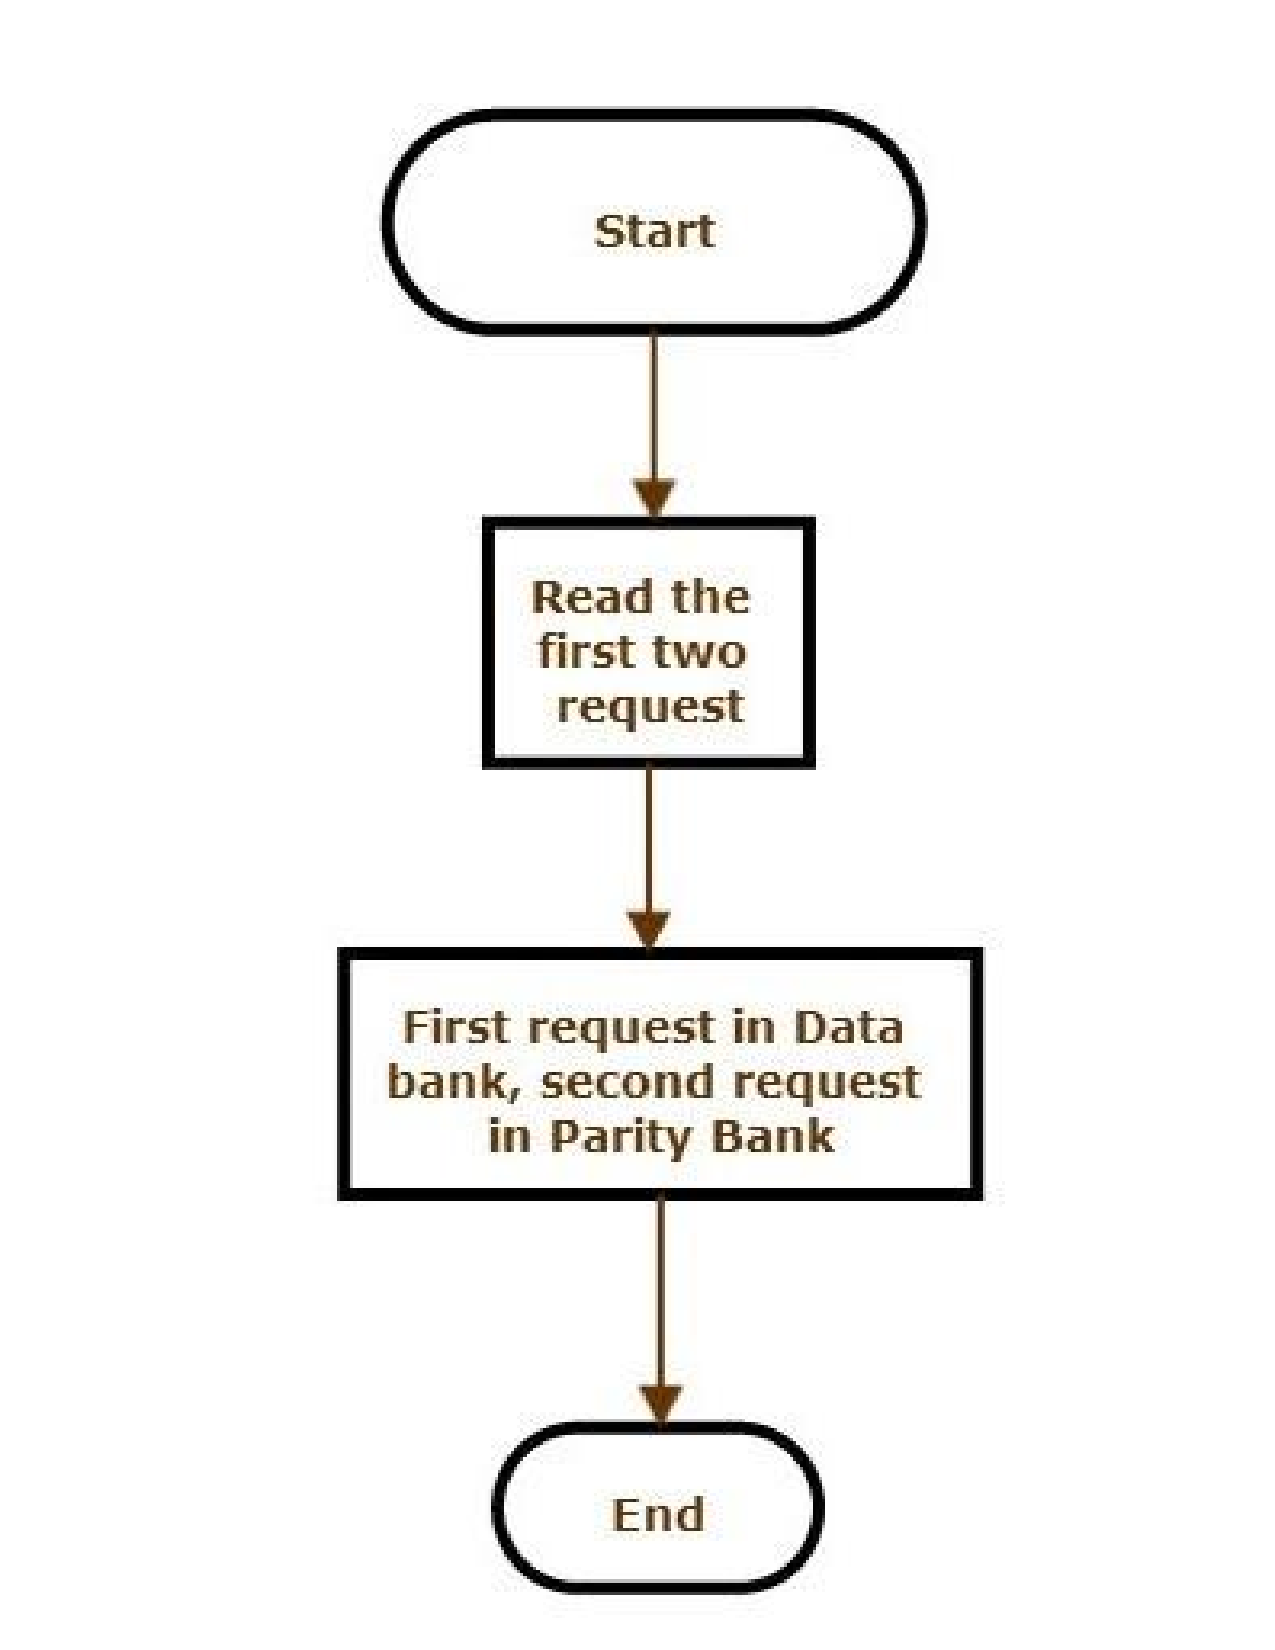
\includegraphics[width=\linewidth]{fig/writealgo.pdf}
	\caption{{\bf Flowchart of Write Algorithm}}
	\label{fig:writeAlgo}
\end{figure}
%-------------------------
%\ignore{
\begin{itemize}
\item Write about how we solve the out of order look ahead problem. If we solve 
	it at all ????
\end{itemize}
}
%\subsection{Write Algorithm for Coded Memory system}
\subsection{Write pattern builder}
\label{sec:writeCodingAlgo}
\Matt{Do we want a flowchart in here to parallel the one in section 4.3?}
Next, we address the issue of scheduling write requests during the operation of the proposed memory system. Recall that the write requests are first filled in the write queues for each bank by the bank arbiter. The unit that resides in the access scheduler and commit these write requests to the memory banks is referred to as {\em write pattern builder}. The write pattern builder waits till a write queue gets full to schedule the write requests to be served. This approach is adopted in order to ensure that the read requests get priority over the write requests.

In particular, we aim to commit $2$ write request per data bank in the given memory cycle. When the write queue for a particular bank gets full, the write pattern builder picks $2$ write request from the head of the queue. It write the first write request to the corresponding data bank. For the other write request to be scheduled, the builder commits this request to one of the parity banks that depend on the data bank associated with the write request. {\color{blue}In particular, the builder replaces the parity element that depends on the data element of the write request with the data element itself. Note that this destroys the parity elements and the coding scheme (in the corresponding row is deemed outdated).} This requires us to update the code status table accordingly. We handle the outdated coding scheme using another block of the access scheduler, namely {\em ReCoding unit} (cf.~Section~\ref{sec:recoding}).

% When a write is scheduled for a particular bank, the scheduler picks up {\bf 
%two} requests from the head of the queue. It writes the first request to the 
%corresponding data bank. The second write is committed to the parity bank of the 
%respective row. Figure ~\ref{fig:writeAlgo} describes the write algorithm as a 
%flowchart. \\

We illustrate the aforementioned functioning of the write pattern builder with the help of an example shown in Figure~\ref{fig:writeAlgoAccessPattern}. In this example, the write queue is full for all the four banks. The controller picks up $2$ write requests from each of these queues and schedules them to be written to the respective data bank and one parity bank. The controller also updates the code status table map with the appropriate status. It updates the writes committed to data bank with $01$ and writes committed to parity bank with $10$. The write build pattern will only serve a write using parity banks if the request's row exists in the parity bank.


\begin{remark}
In the example described in Figure~\ref{fig:writeAlgoAccessPattern}, the queues for all data banks become full at the same time. In general, this is not the case and the write queues for some of the data banks become full before it does so for the other data banks. In this case, the write requests for only some of the banks get scheduled in a given memory cycle.{\color{blue} We note that the controller is designed to schedule both read and write for each bank depending on 
the queue size and availability of the parity of banks. Therefore, if a data bank is not utilized to serve a write request in a memory cycle, it can be potentially utilized to serve a read request in that cycle.} \Matt{The current simulations only schedule reads requests OR write requests in a single memory cycle. There are issues in Ramulator when scheduling reads and writes simultaneously...}
\end{remark}

\begin{remark}
An exception to the standard logic of the write pattern builder is invoked when the accesses are linear in nature for all $4$ data banks. For example, if we have write requests for the elements $a(1), b(1), c(1),$ and $d(1)$. In such a case, the controller directly updates all the parity banks by writing the updated versions of the parity elements $a(1) + b(1), a(1) + c(1), a(1) + d(1), b(1) + c(1), b(1) + d(1),$ and $c(1) + d(1)$. This ensures that the parity banks remain updated and the 
memory controller no longer need to update the parity bank using ReCoding unit (cf.~Section~\ref{sec:recoding}). The reason for invoking this exception is to avoid the extra cost involved in recoding the whole row. Though this saving in the cost of recoding come at a price as we fall back to $1$ write request per data bank in the underlying memory cycle. 
\end{remark}

%Figure~\ref{fig:writeAlgoAccessPattern} describes the writes algorithm with an example.
%The write is selected for a bank when the write queue is full. The scheduler picks up two 
%elements from each bank for writes. It schedules the first element to be written to the data bank
%and the second one to be written to the memory bank. The memory controller updates the code status map 
%according to table~\ref{table:codestatusmap}. For elements stored to the data bank, i.e., the first element,
%it updates it to {\bf 01} and for elements stored in parity bank to {\bf 10}.
\ignore{writes are scheduled to address {\em a2} and {\em a9}. The write to {\em 
	a2} goes to {\em a2}, however, the write to {\em a9} goes to the data 
bank {\em a9 + b9}. This helps us do two writes in one cycle.  However, the 
databank of {\em a9} still contains the stale value. The scheduler updates the 
{\em coding status} of each row after committing a write. }
%-----------------------
\begin{figure}[t!]
\centering
	%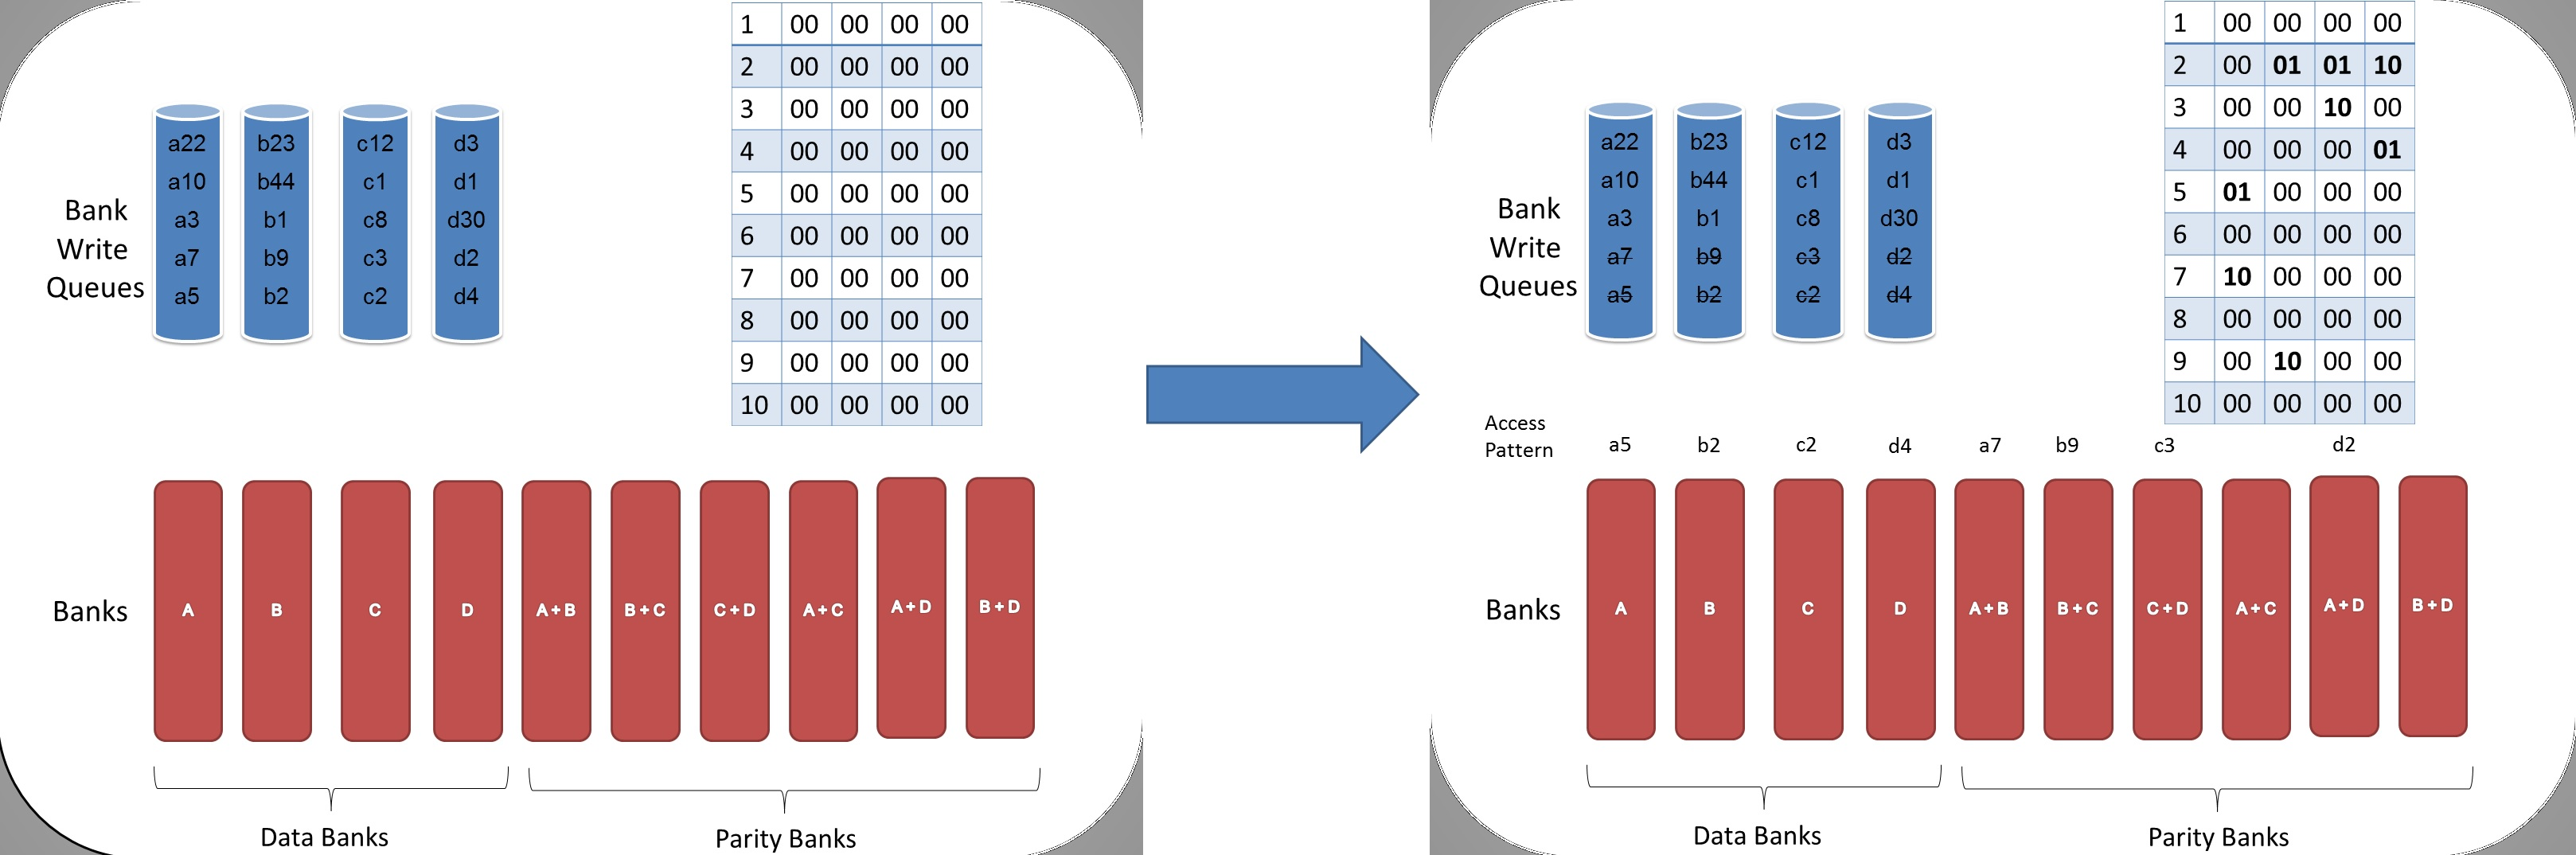
\includegraphics[width=\linewidth]{fig/writeAlgoAccessPattern.jpg}
         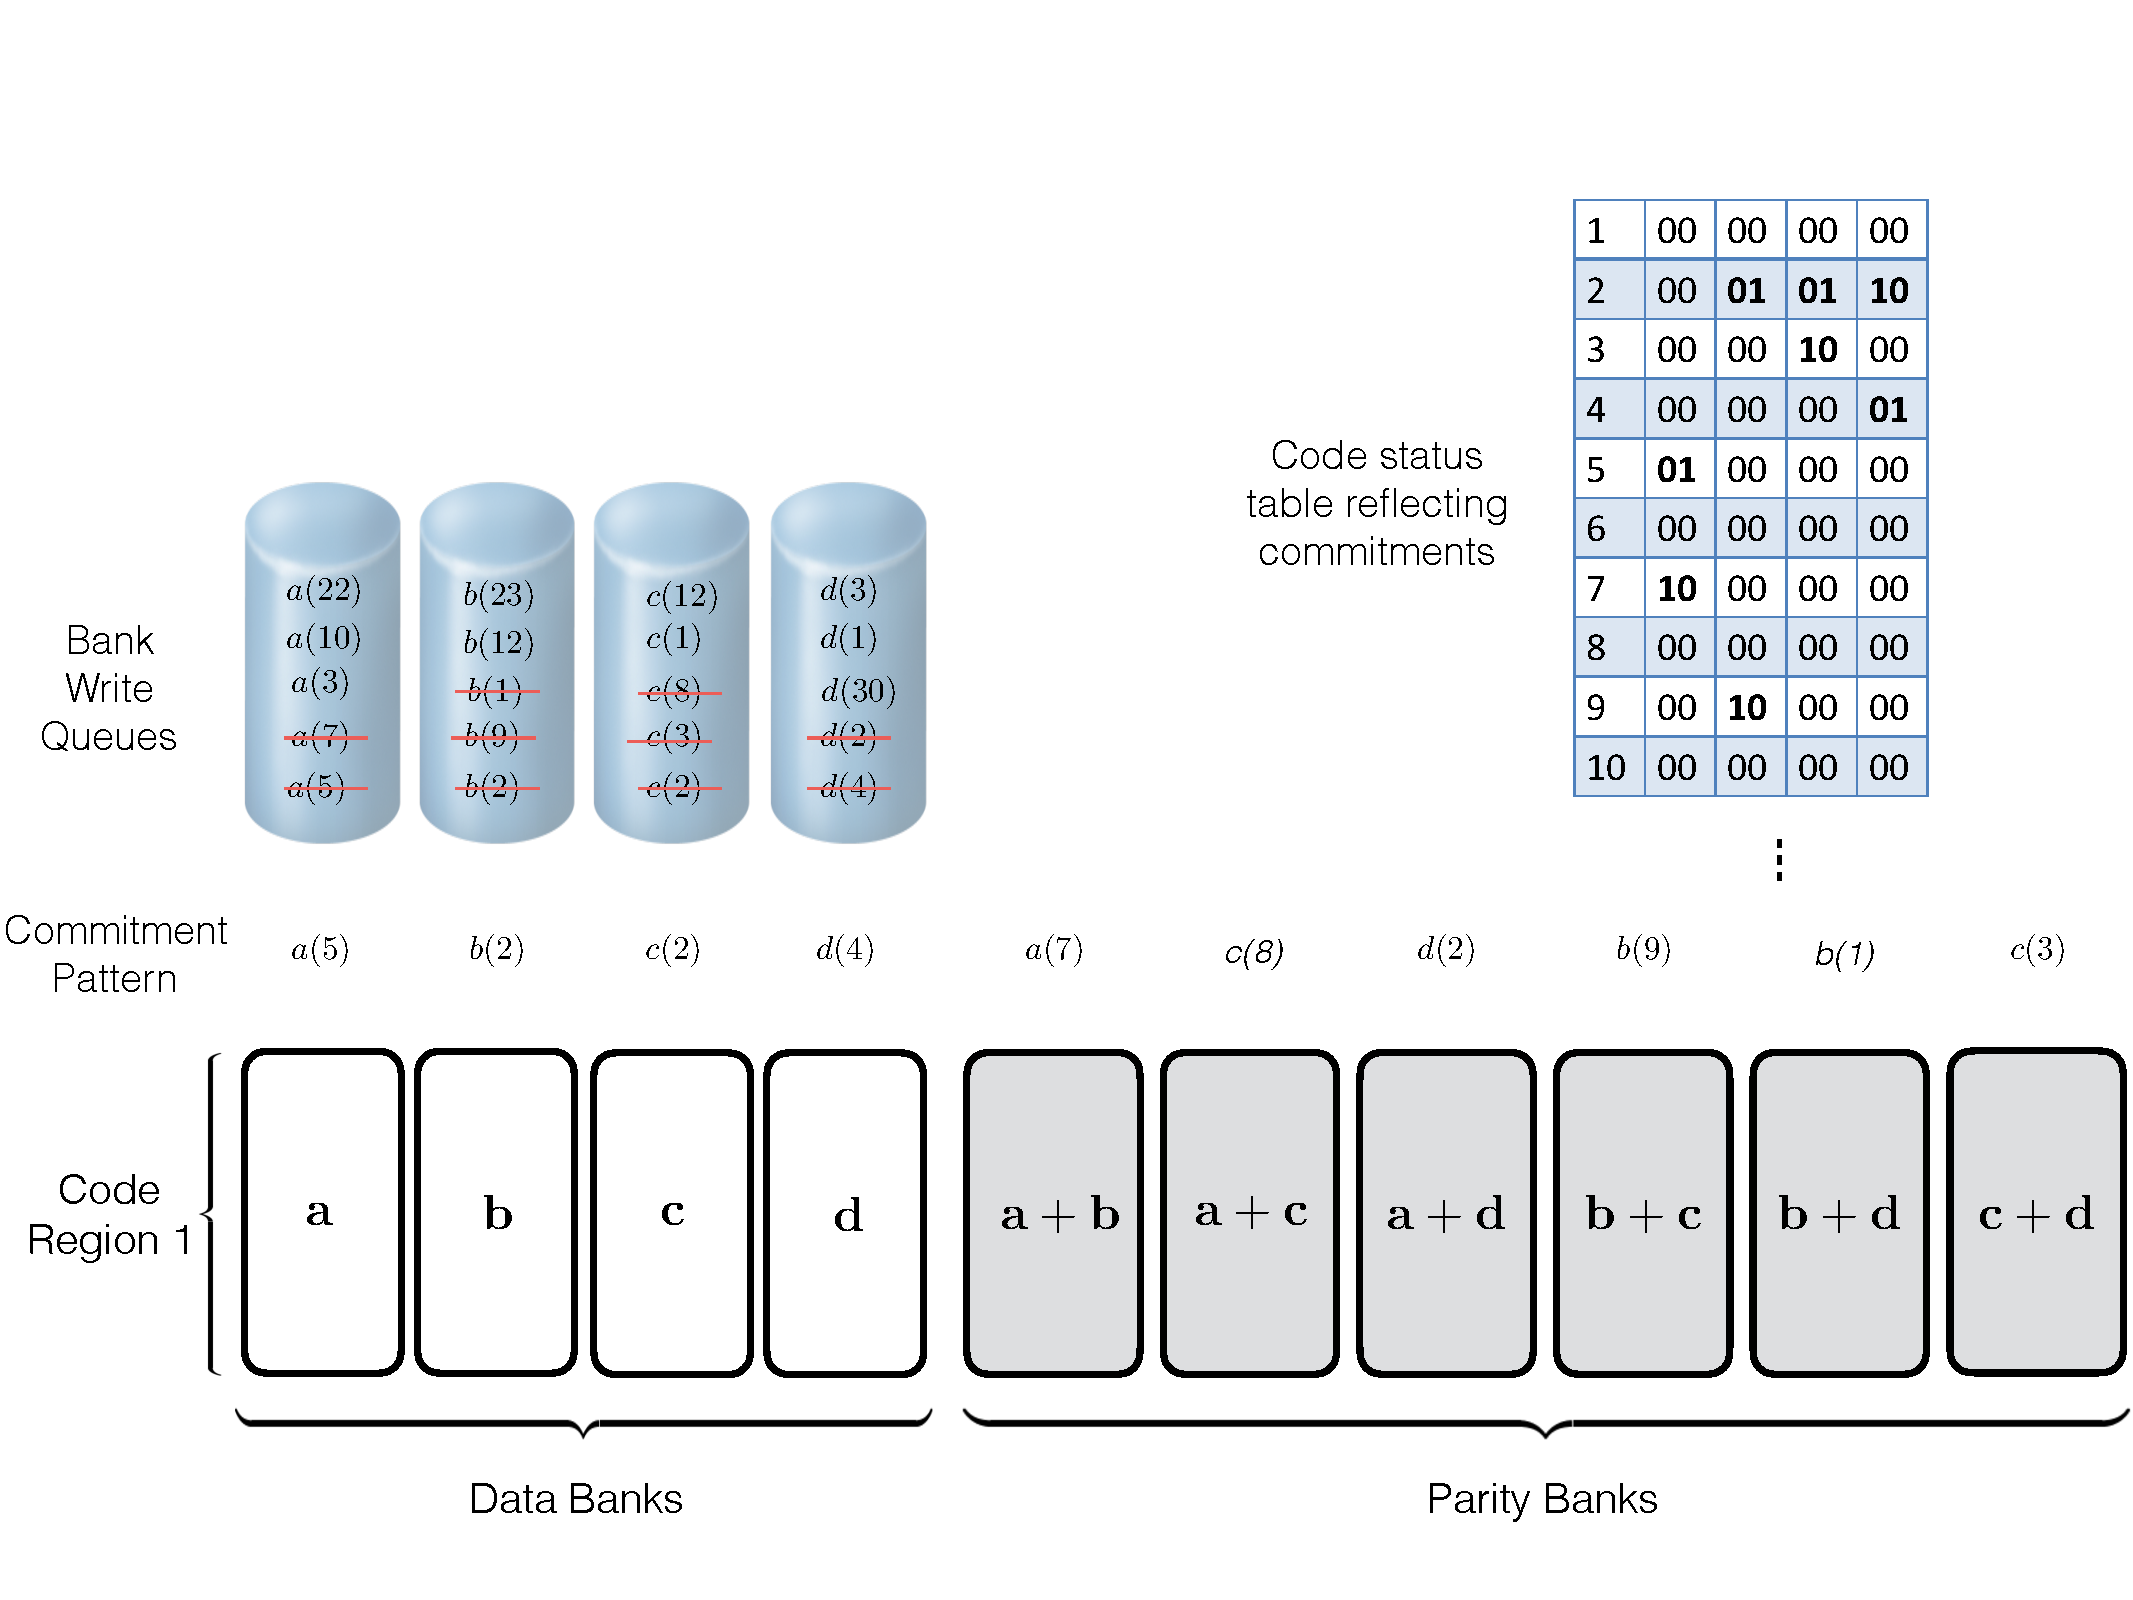
\includegraphics[width=\linewidth]{fig/Write-Algo-Example.pdf}
	\caption{Figure describing write algorithm access pattern}
	\label{fig:writeAlgoAccessPattern}
\end{figure}
%-------------------------
\subsection{ReCoding unit}
\label{sec:recoding}
As described in Section~\ref{sec:writeCodingAlgo}, committing write requests to the memory banks destroys the coding scheme for the corresponding row. Note that this information is available in the code status table. In order to maintain the original (coded) storage so that it can be utilized to reduce the latency experienced by the read requests, the memory controller needs to restore the coding scheme with the updated values of data elements.
%It then implies a requirement to the memory controller to restore the code back with the updated values. 
The ReCoding unit is responsible for recoding the updated rows at a later time. This unit  comprises a queue which holds the row number of the updated code. Each row in the queue is associated with the cycle number or a counter which serves as a timing notion of how old is the request in the queue. The controller can be designed to recode a row within {\color{red}XYZZZZZ} number of cycle after its update. 

The ReCoding unit restores the coding scheme by utilizing banks left idle by the read and write pattern builders. In the case of restoring data in a parity bank, the ReCoding unit downloads and stores from the data banks over one or more memory cycles and restores the parity code once all requisite data has been retrieved. For storing a write which has been stored in a parity bank, the ReCoding unit writes the new data to the parity bank and then begins to restore the parity code. If in the execution of the read and write pattern builders data which is useful to the ReCoding unit is accessed, the data is sent to the ReCoding unit.


\subsection{Dynamic Coding}
\label{sec:dynamicCoding}
The {\em dynamic coding} block in the access scheduler is responsible for 
maintaining codes for heavily accessed memory sub regions. This block primarily 
helps in the reduction of code storage for unused memory. This algorithm finds 
out the current heavily accessed region and indicates to the controller to code 
that region. With this, we require only a fraction of the whole memory to be 
coded.  

The contention in memory accesses from various cores occurs mostly when the 
access are to shared-memory, especially when they are localized to certain 
memory regions. We explore the locality of the memory access over a period of 
time to reduce the memory overhead for storing the codes. In a multi-core 
system, when various cores try to work from a shared memory location, they tend 
to generate accesses to a localized region of memory. This motivates the idea of 
coding the localized region during the period of heavy access, and dynamically 
changing the region whenever there is change in the locality of memory accesses.
Figure~\ref{fig:dedup_whole} shows the access pattern for cores 0 to 7 running the dedup PARSEC benchmark.  
The y-axis of the figure shows the address accessed by the coress over a 
period of time. The x-axis denotes the time in nanoseconds. This plot shows that 
most of the access from various cores are primarily located in the lower memory band. Greater than 95\% of all memory accesses are from this band ~\ref{fig:dedup_dense} magnifies this band and reveals that the lower band is composed of two subbands of roughly equal density.

\begin{figure}[htbp]
		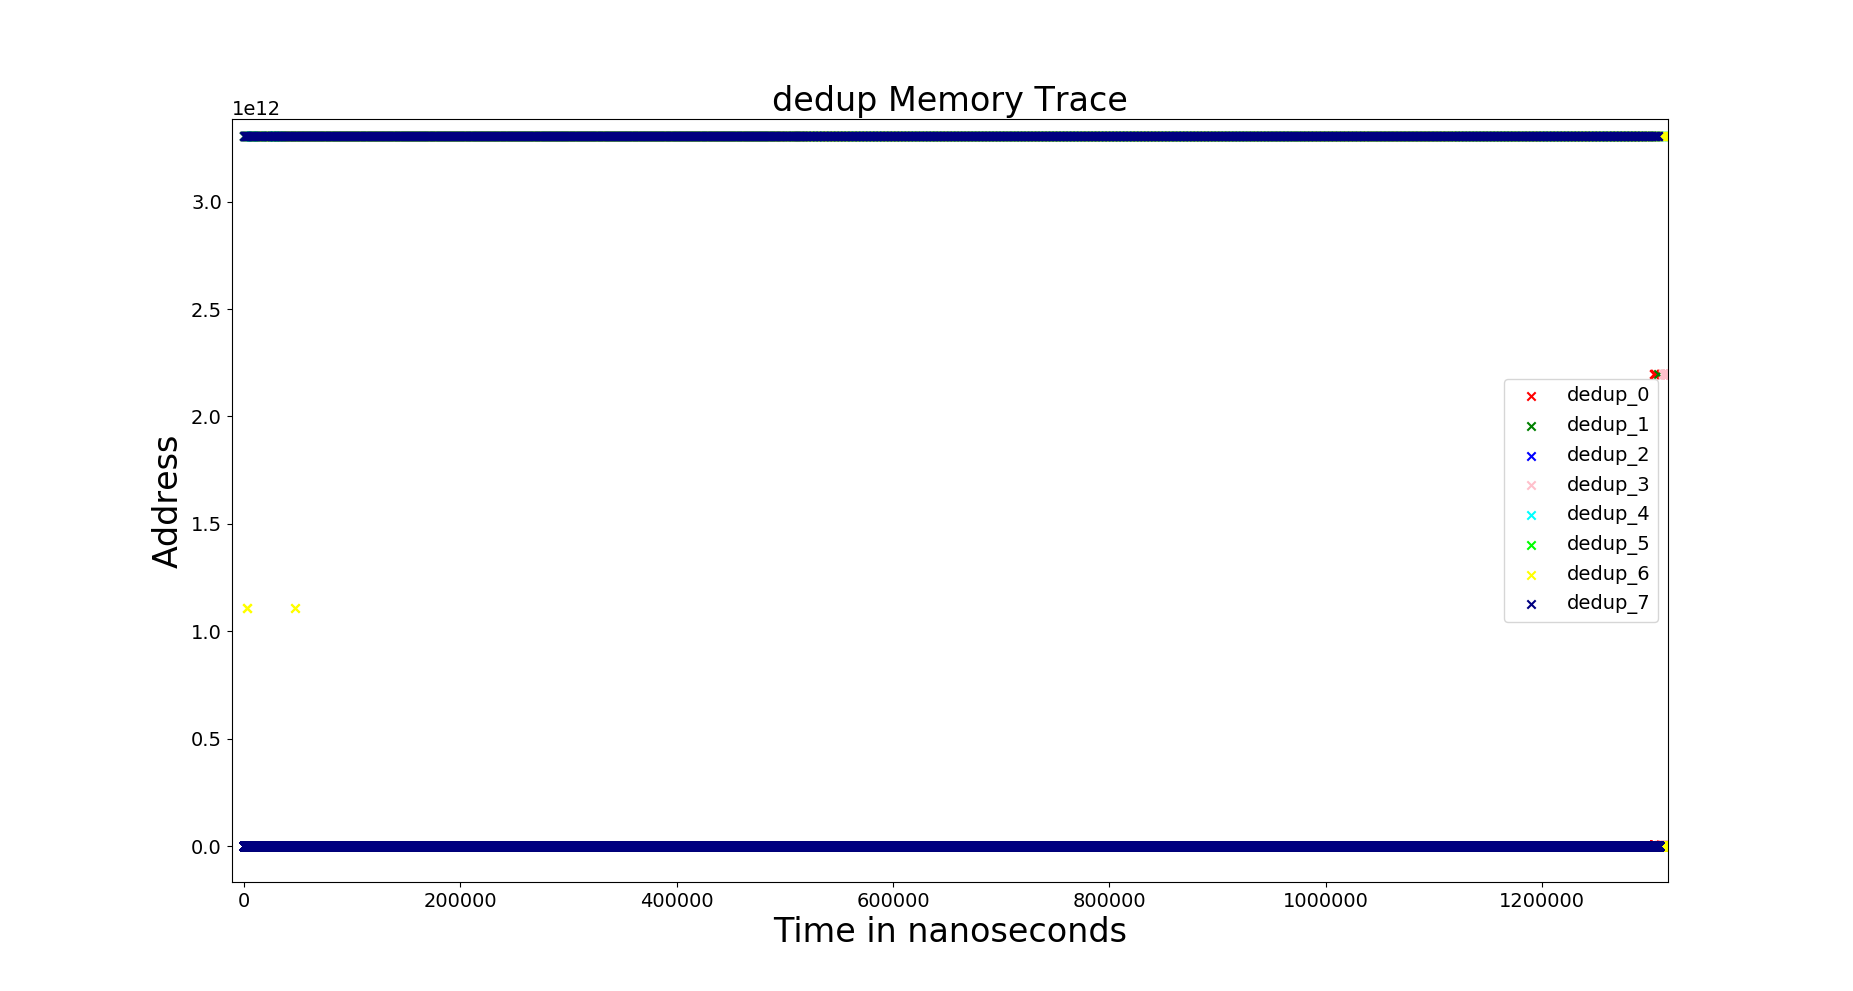
\includegraphics[width=\linewidth]{fig/dedup_whole.png}
		\caption{Memory Access from the Dedup PARSEC benchmark. This trace was generated using 8 cores.}
		\label{fig:dedup_whole}
\end{figure}

\begin{figure}[htbp]
		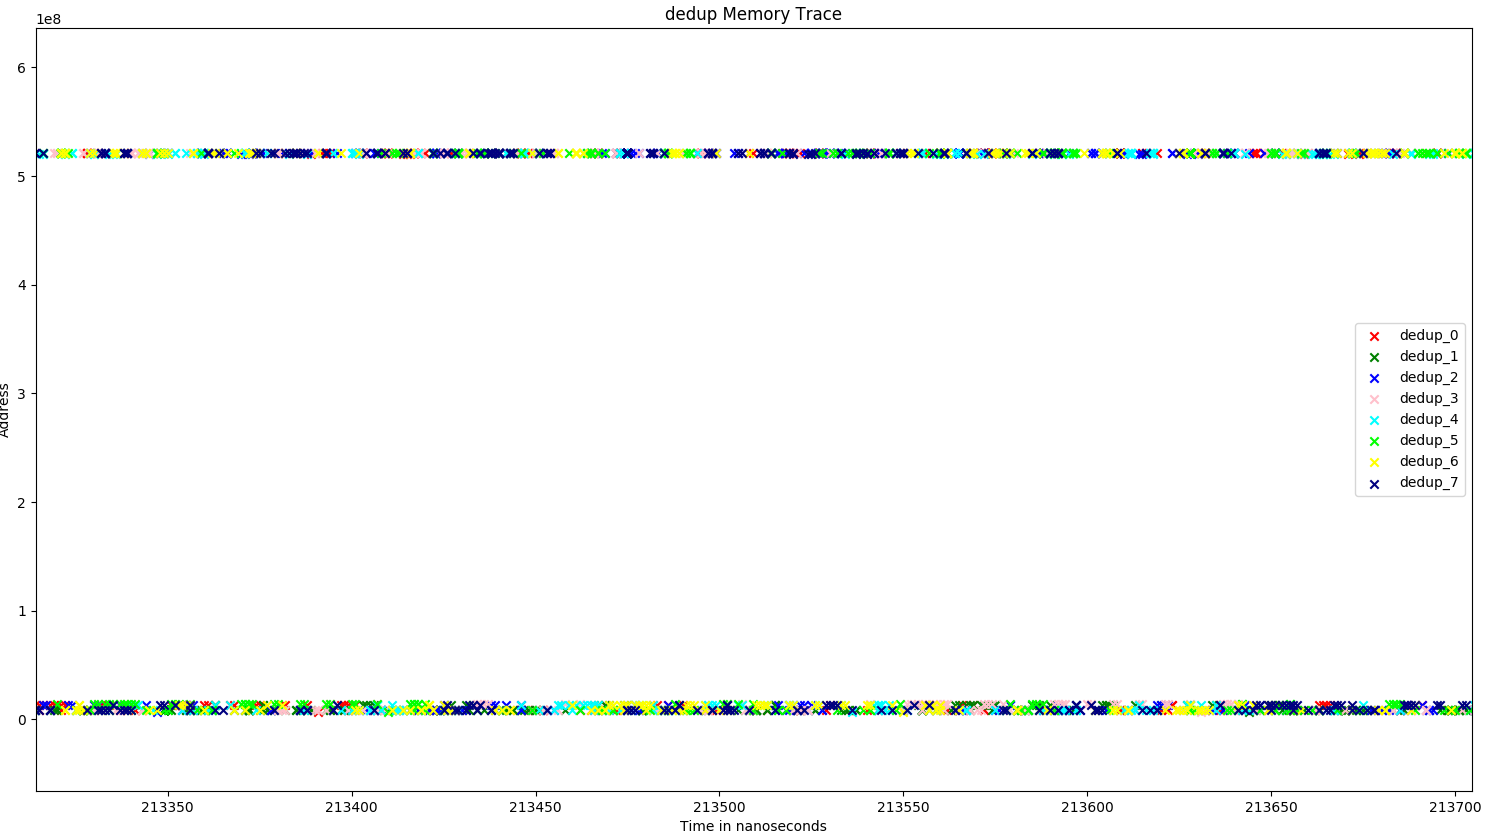
\includegraphics[width=\linewidth]{fig/dedup_dense.png}
		\caption{Memory Access from the Dedup PARSEC benchmark demonstrating the density of memory accesses}
		\label{fig:dedup_dense}
\end{figure}

From the above observations, we demonstrate the idea of coding the 
highly accessed portion of the memory. This scheme benefits from a huge 
reduction of the memory overhead with coding. The reduction in the memory 
overhead can be used to reduce the complexity of the decoder by using simple 
coding functions (e.g. xor) and for denser coding (e.g. repeatedly coding a 
single element using 2 elements). 

The scheme of dynamic coding requires that the currently coded region changes 
when the access pattern changes. That is, the localized memory area that is most heavily accessed 
can change, and it will require the system to recode the new localized access 
region. We assume that the working area of a program changes with change in the 
input parameters to the program. It can be easily observed from the above 
figures that the working area or the localized area is constant for at least 1 
ms. This suggests that the switching of the coded region is not very frequent. 
%{\bf During these periods of coding switches, it is also guaranteed that the number 
%of accesses served from the memory is at worst equal to the number of banks 
%available. In other words, coding the memory has no performance degradation 
%compared to non-coding during these times.} The system also needs to maintain an 
%algorithm to observe the access pattern of the cores, and make a decision when 
%it is time to code a new memory region. To do this, the memory controller tracks 
%the most accessible region during a time period and makes a decision to 
%slide/shift the coded region. This shift in the coded region requires the update 
%of the parity bank for the new region. This process is carried out in 
%conjunction with the ongoing access to the newly coded region. Therefore, this 
%operation only requires writes to the parity banks, since we can use the current 
%reads from the coded region to access the data that is to be coded. In addition, 
%reads are also scheduled in the idle periods, when there is no read or write 
%request to the bank/banks.\\
{\em Dynamic coding} requires the system to divide the memory into sub-regions and to 
keep track of accesses in these sub-regions. Once the number of accesses to a 
sub-region reaches a given threshold, it must then make this region the 
currently coded area. We propose this mechanism based on window concept. The 
system maintains a tuple of sub-regions such as [Starting Address, Length]. Each 
sub-region is thus given a starting address and length. Any access to a 
particular sub-region is considered as a hit. The system has a hit counter 
associated with each of the sub-region which is incremented for each hit. The 
system makes a decision of coding a particular sub-region based on its counter 
value. The number of coded sub-regions at a particular time is based on the 
sub-region size and the code storage size. The eviction of a coded region 
follows the Least Recently Used (LRU) policy similar to cache.

The block implements a simple logic to determine heavy access to a particular 
region. It divides the whole memory in to subregions. The memory can be 
divided dynamically with the provision of the following window parameters 
\{StartAddress,Length\} . The controller can have multiple window parameters 
with the constraint that the total length should be less than the available 
memory for code storage. This would allow the system designer to have small 
chunks of distributed memory to be coded. It is important to note here that the 
codes described are obtained by linear combination of data elements of the same 
row in various memory bank. So, essentially the window parameter for address 
signifies the row start.

The {\em dynamic coding} block splits the each memory bank according to the memory partition coefficient {\em r}. Each bank is split into $\lceil\frac{1}{r}\rceil$ partitions. The block can select up to $\frac{\alpha}{r} - 1$ regions to be encoded in the parity banks. A single region is reserved to allow the dynamic coding block to encode a new region.

Every $T$ ticks, the {\em dynamic coding} block chooses the $\frac{\alpha}{r} - 1$ regions with the greatest number of memory accesses. The block will then encode these regions in the parity banks. If all the selected regions are already encoded, theblock has nothing to do. Otherwise, the block begins encoding the regions in order of most accesses. Once the block is finished encoding a new region, the region becomes available for use by the rest of the memory controller. If the memory ceiling $\alpha - r$ is reached when a new memory region is encoded, the {\em dynamic coding} block evicts the least frequently used memory region. 

The dynamic coding controller resets the count of access to the subregions at 
the switch of the subregion. The new counts determine the next change of the 
coded subregion.

%\ignore{
\subsection{Prefetching Codes}
\label{sec:prefetching}
The technique of dynamic coding reduces the memory overhead by exploiting the 
localized nature of memory accesses from the cores. In this section, we explore 
prefetching the coded data to reduce the access overhead caused for fetching the 
codes. This is done by exploiting the gaps in the memory access to any bank and 
using these gaps to prefetch the code/data for a future memory access. During a 
program, there are access cycles when certain banks do not have any access 
scheduled for a read/write. We propose the prefetching technique where we look 
forward in the queue and anticipate a pre-fetch for the data/code for that bank.  
We explore the implementation of a memory prefetching unit, similar to an 
instruction or cache prefetching unit. This unit can detect linear access 
patterns to regions in memory.  For example, if a string of memory accesses are 
issued in sequential byte sized order, then the prefetching unit will predict 
the next access to be in byte increments. The memory prefetching works by 
fetching a predicted address from the parity bank during accesses that the 
parity bank is idle. When future memory accesses are issued, they are first 
checked with the pre-fetched data to see if they can be used to decode any 
subsequent memory accesses. If so, the memory access is obtained from the 
current accesses and pre-fetched data. For example, say the pre-fetcher sees 2 
consecutive memory requests in a row. It then predicts that the next two 
accesses, locations $a_0$ and $b_0$, are likely to be accessed in the near 
future. It reads $a_0+b_0$ from the parity bank for future use. Next, access to 
location $a_0$ and $b_0$ are issued to the memory. Now, instead of reading both 
$a_0$ and $b_0$, only a single location has to be read from in memory, while the 
other location can be obtained from the pre-fetched data. This allows for an 
additional access to be issued from the now free memory bank.  In these cases, 
it is possible to obtain up to two additional memory accesses in a given cycle, 
one from the pre-fetched data and one from the parity bank.
\begin{figure}[htbp]
\centering
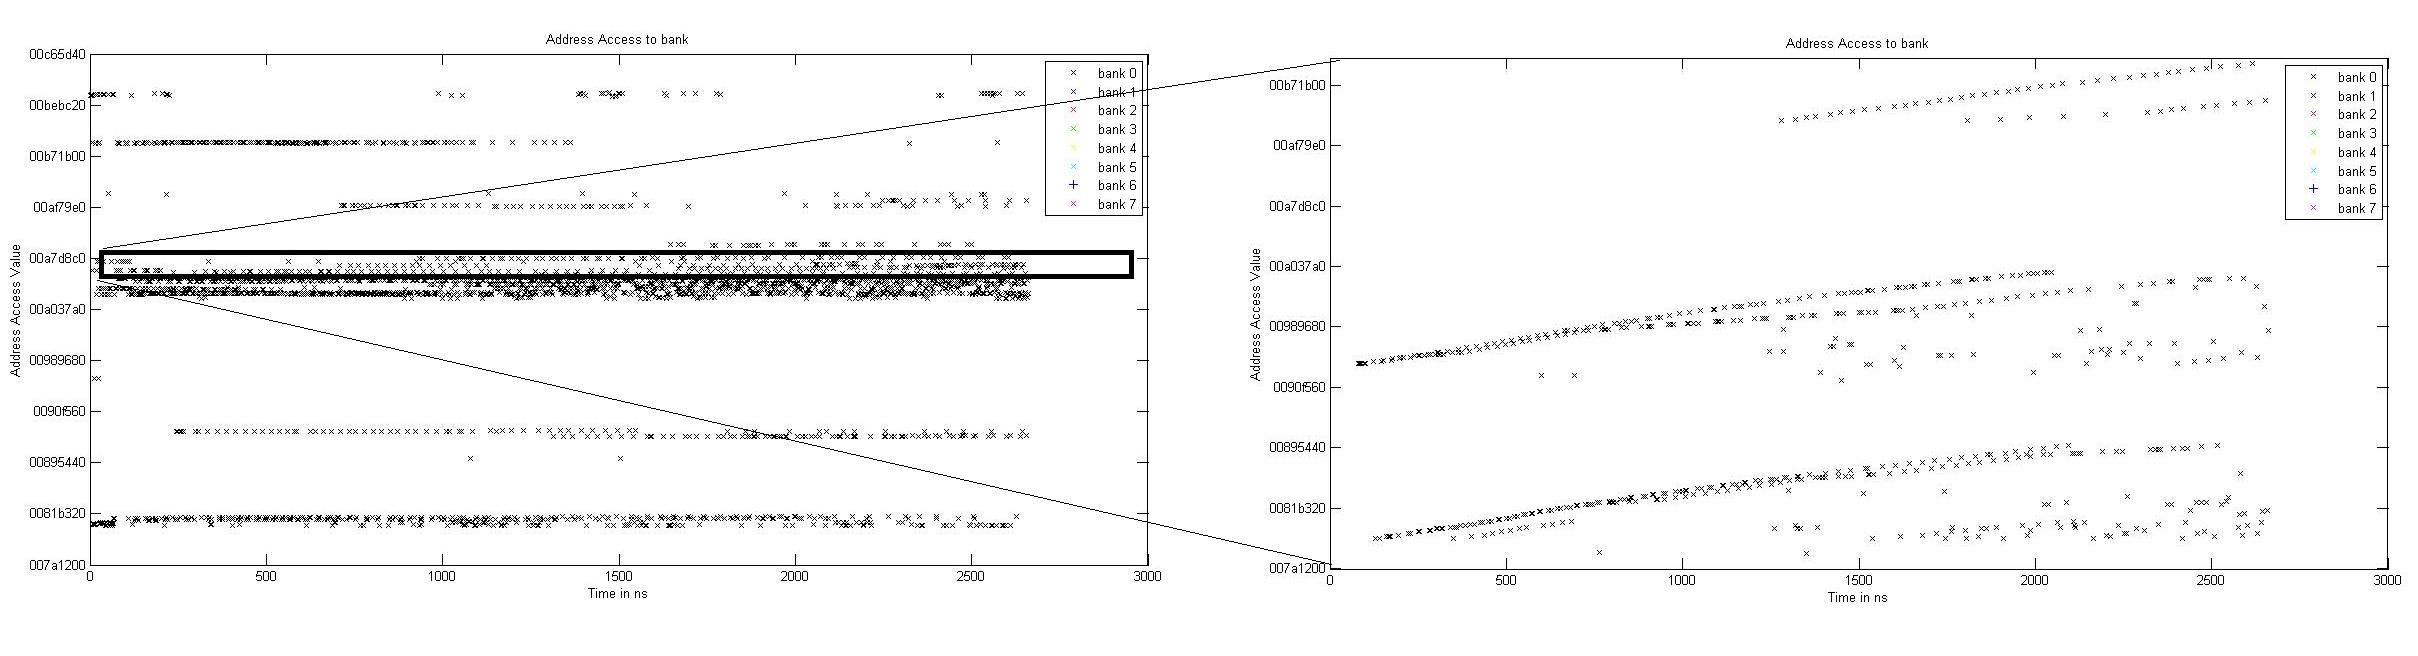
\includegraphics[width=0.5\linewidth]{fig/bank_access1.jpg}
\caption{ }
\label{fig:bank_access1}
\end{figure} Implementation of a memory prefetch should only require overhead 
for space and the associated logic to implement it. Since memory accesses are 
often stalled due to bank conflicts, checking pending accesses to the 
pre-fetched data should require no additional time overhead. As memory accesses 
wait to be issued in the bank queues, they can simultaneously be checked with 
the pre-fetched data. Thus, no extra latency is anticipated by the addition of a 
memory prefetching unit.
Figure~\ref{fig:bank_access1} shows two plots of memory accesses to a bank with 
respect to time. The left figure shows the accesses to the memory bank by 
various cores. The right side figure shows a zoomed view of the accesses in the 
dense access region. This figure suggests the linearity of accesses. The system 
can look ahead in the queue to detect the consecutive address request for a 
memory bank and schedule a prefetch of the associated code.  In 
figure~\ref{fig:queue_lookahead}, we simulate the prefetching of the code by 
using a window of length ??. That is, we look ahead to ?? requests in the queue 
and find out the occurrence of consecutive address in the window. The plot 
suggest high occurrence of the consecutive addresses in the bank which can be 
served by prefetching the codes.  
%-----------------------------------
\begin{figure}[htbp]
\centering
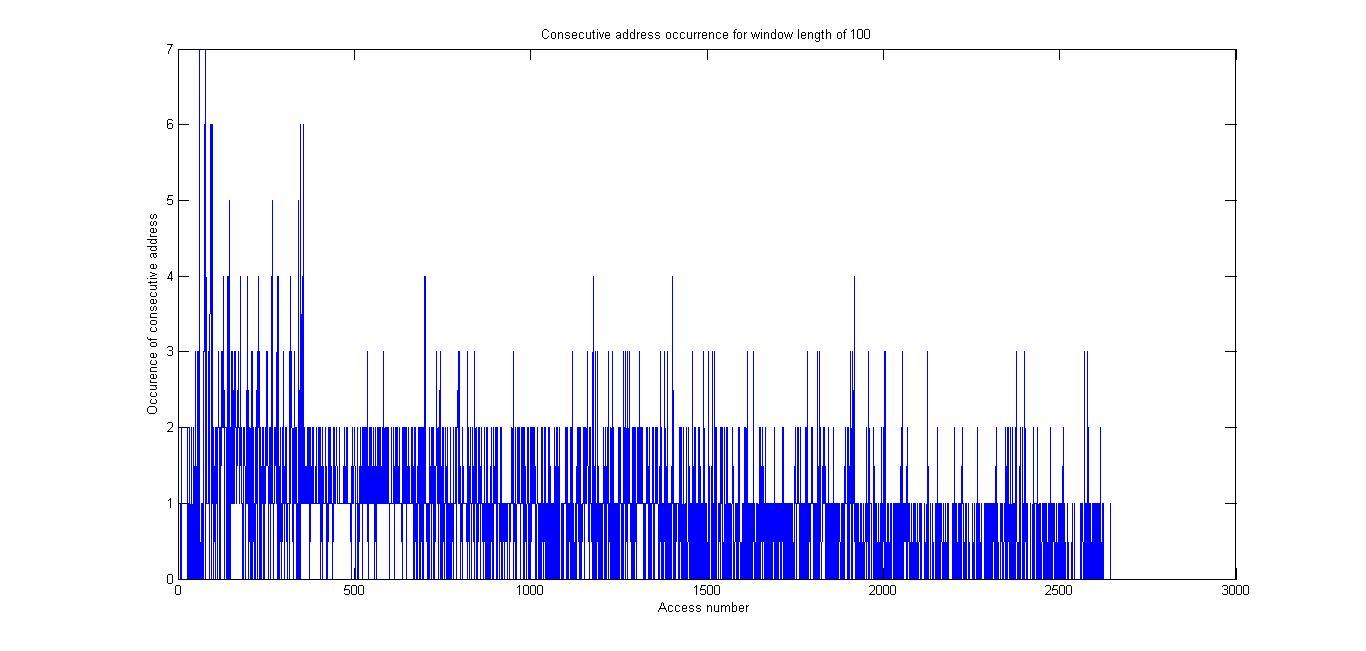
\includegraphics[width=\linewidth]{fig/queue_lookahead.jpg}
\caption{ }
\label{fig:queue_lookahead}
\end{figure} 
%-----------------------------------
%}
%\ignore{
 
%}
